% Settings
\newcommand{\doctitle}{Efficacy Of Dose Painting On Uncertain Biological Tumor Maps\\For Head And Neck Cancer Treatment}
\newcommand{\doctype}{Master Thesis}
\newcommand{\thesisauthor}{Alexander Runde}
\newcommand{\matriculation}{123456}
\newcommand{\academicyear}{2011/2012}
\newcommand{\supervisor}{Prof. Dr. Uwe Oelfke}
\newcommand{\cosupervisor}{Dr. Emily Heath \& Dr. Harald Keller}
\newcommand{\degree}{Master Degree in Physics}
\newcommand{\university}{Ruperto-Carola University of Heidelberg, Germany}
\newcommand{\department}{German Cancer Research Center, Heidelberg}
\newcommand{\logo}{contents/images/university_logo.png}
\newcommand{\logowidth}{0.5 \linewidth}

% Style Settings

% - Document Class
%\documentclass[dvipdfm,11pt,letterpaper,twoside,openright,english]{book}
\documentclass[pdftex,11pt,letterpaper,twoside,openright,english]{book}
% - ToC Depth
\setcounter{tocdepth}{2}
% - ToA Style
\newcommand{\tableofacronymstyle}{longheaderborder}
% - References Style
%\newcommand{\mybibstyle}{ieeetr}
\newcommand{\mybibstyle}{unsrt}

% Packages
\usepackage{amsmath}
\usepackage{amsfonts}
\usepackage[pdftex]{graphicx}
\usepackage{xfor}
\usepackage[T1]{fontenc}
\usepackage{ae,aecompl}
%\usepackage[nonumberlist,acronym,toc]{glossaries} 
\usepackage{longtable}
\usepackage{multirow}
\usepackage{setspace}
\usepackage[hyphens]{url}
\usepackage{cite}
\usepackage{setspace}
\usepackage{float}
\usepackage{epigraph}
\usepackage[english]{babel}
\usepackage[belowskip=-10pt,aboveskip=0pt]{caption}
\usepackage{rotating}
\usepackage{booktabs}
\usepackage{subfigure}

% Pages layout
\usepackage[top=35mm, bottom=25mm, left=35mm, right=35mm]{geometry}

% Enable glossaries
%% Uncomment if you want to display all the entries (and not just the referenced ones)
\glsaddall
%
\newglossaryentry{Abcdefz}{name=Abcdefz,description={An \emph{abcdefz} is a Lorem ipsum dolor sit amet, consectetur adipiscing elit. Curabitur pharetra venenatis odio, ac pellentesque nulla blandit at. Maecenas eget massa arcu. Duis tempor justo et sapien ornare pulvinar}}
\newglossaryentry{Acderds}{name=Acderds,description={An \emph{acderds} is a Lorem ipsum dolor sit amet, consectetur adipiscing elit. Curabitur pharetra venenatis odio, ac pellentesque nulla blandit at. Maecenas eget massa arcu. Duis tempor justo et sapien ornare pulvinar}}
\newglossaryentry{Bpoiwne}{name=Bpoiwne,description={A \emph{bpoiwne} is a Lorem ipsum dolor sit amet, consectetur adipiscing elit. Curabitur pharetra venenatis odio, ac pellentesque nulla blandit at. Maecenas eget massa arcu. Duis tempor justo et sapien ornare pulvinar}}
\newglossaryentry{Csdfdse}{name=Csdfdse,description={A \emph{csdfdse} is a Lorem ipsum dolor sit amet, consectetur adipiscing elit. Curabitur pharetra venenatis odio, ac pellentesque nulla blandit at. Maecenas eget massa arcu. Duis tempor justo et sapien ornare pulvinar}}
%
%
\newacronym{ABC}{ABC}{Lorem ipsum dolor}
\newacronym{DEF}{DEF}{Lorem ipsum dolor}
\newacronym{GHI}{GHI}{Lorem ipsum dolor}
\newacronym{LMN}{LMN}{Lorem ipsum dolor}
%
%\makeglossaries

% Interline
\linespread{1.4}

% PDF properties
%\hypersetup{
%colorlinks=false,
%linktocpage=true,
%plainpages=false,
%pdfborder=0 0 0,
%bookmarksopen=true,
%pdftitle=\doctitle,
%pdfauthor=\thesisauthor
%}

% Set initial pagenumbering to none
%\setcounter{page}{0}
\pagestyle{empty}

% Indented Paragraph ;) - Use it like \begin{indentparagraph}{3cm}{your-paragraph}\end{indentparagraph}
\newenvironment{indentparagraph}[1]{\begin{list}{}{\setlength{\leftmargin}{#1}}\item[]}{\end{list}}
\newcommand{\specialcell}[2][c]{%
\begin{tabular}[#1]{@{}c@{}}#2\end{tabular}}

%hyperref
\usepackage[pdftex, plainpages=false, pdfpagelabels]{hyperref}
\begin{document}

\thispagestyle{empty}
\begin{center}
    \vspace{8mm}
    {\includegraphics[width=\logowidth]{\logo}} \\
    \vspace{8mm}
    {\large \university} \\
    \vspace{8mm}
    {\large \department} \\
    {\large \degree} \\
    \vspace{8mm}
    {\large \doctype} \\
    \vspace{10mm}
    {\large\bf \doctitle} \\
    \vspace{8mm}
    {\large Author \\ {\bf{\thesisauthor}} \\ Matr. \matriculation }\\
    \vspace{10mm}

    \begin{tabular}{c  @{\hspace{2.5cm}} c}
    Supervisor & Co-Supervisors \\
    \bf{\supervisor} & \bf{\cosupervisor} \\
    \end{tabular} \\

    \vfill
    {\large Academic Year \\ \academicyear} \\
\end{center}
\newpage

\cleardoublepage

\null\vspace{\stretch{1}}
\begin{flushright}
{\it{
I dedicate my work to my family. \\
You gave me the support to make a \\
difference in other peoples lives. \\
- \\
I love you \\

}}
\end{flushright}
\vspace{\stretch{2}}\null
\newpage
\cleardoublepage

\chapter*{Abstract/Zusammenfassung}{% abstract

\textit{Dose painting} is a new way to incorporate imaging of tumour biology into treatment planning to improve the efficacy of radiation therapy.  Hypoxia has been identified as one of the major reasons for the failure of local tumour control in head and neck cancer. The lack of oxygen enhances DNA repair from radiation damage, which leads to higher radioresistance in such hypoxic tumour regions. Dose painting can help to overcome hypoxia by increasing the dose to account for higher radioresistance. This thesis will introduce a new way of dose painting using the biological effect (\textit{biological dose painting}) to overcome the treatment deficiencies created by hypoxia. Ten head and neck cancer patients with clinically approved plans from the Princess Margaret Hospital (Toronto, Ontario, Canada) have been used to apply biological dose painting under iso-toxic treatment planning to show feasibility of the new approach. Afterwards the deployed models are examined in terms of their model parameter uncertainties to assess the robustness of biological dose painting. This work shows, that biological dose painting is feasible and compensates for changes in radioresistance caused by hypoxia. All critical structures are spared according to clinical constraints while hypoxic volumes receive an appropriate dose to compensate for higher radioresistance.}
\thispagestyle{empty}
\cleardoublepage

\chapter*{Acknowledgements}{%
I would like to express my gratitude to everyone who has supported my in one or the other way during the course of this master thesis. I would like to thank Prof. Dr. Uwe Oelfke for providing me with a very interesting and challenging topic as well as for providing an exceptional working environment at the DKFZ.\\I would like to thank Prof. Dr. Emily Heath for her support as well as for her invitation to work in Toronto with her for four months. I am very grateful for the financial support that she provided the make this possible as well as her insight into the topic, which made my research a lot easier. In the same instance I would like to thank Dr. Harald Keller from the Princess Margaret, who has supported me greatly during my stay in Toronto and gave me some valuable hints on treatment planning and my thesis.\\Furthermore I would like to thank Dr. Malte Frese for his initial help with my work as well as his insight on further aspects of the topic of this thesis. I also want to thank David J. Carlson, Ph.D., for lending his research date on the topic of hypoxia reduction factors that helped me greatly with the further investigations.\\In addition I would like to thank all my colleagues at DKFZ, especially Dr. Simeon Nill for his kind help with KonRad and other technical problems.\\I want to thank my family for their support and love, which has helped me a lot to pursue this thesis.}
\thispagestyle{empty}
\cleardoublepage

\newpage
\setcounter{page}{1}
\pagenumbering{Roman}
\pagestyle{headings}

\renewcommand{\contentsname}{Table of Contents}
\tableofcontents
\cleardoublepage

\newpage
\setcounter{page}{1}
\pagenumbering{arabic}

\chapter{Introduction}\label{chapter:1}
The term \textit{dose painting} has been around since the year 2000 and has been coined by \textit{Ling et al.} \ref{pmid10837935}. It describes a method of merging biological imaging and treatment planning to increase local tumour control with the help of biological input parameters derived from tumour maps. Such maps are generated from functional images acquired through positron emission tomography (PET) or magnetic resonance imaging (MRI). The biological parameter which is mapped with PET depends on the radiopharmaceutical, which is administered into the patient. While FDG is used to show the metabolic state of the tissue \cite{pmid16841141}, FMISO is currently used as a hypoxia tracer in clinics to spot hypoxic volumes and incorporate them into treatment planning by increasing the dose in these volumes by an arbitrary dose value. One of the major drawbacks when linking the biological image information from PET to a biological tumour map is the ignorance toward to a proper interpretation of image data. Multiple approaches to dose painting have been proposed: Binary dose painting \cite{pmid20855118, pmid11240261, pmid17869020}, functional dose escalation \cite{pmid12587912, pmid21356478, pmid20643512, pmid18635895} and via an implementation of kinetic models \cite{pmid17448882}. With the exception of the latter, all dose painting approaches do not incorporate any biological motivation for the prescription function used to increase the dose in hypoxic volumes. \textit{Bentzen et al.} \cite{pmid19218733} showed how different prescription functions affect the resemblance of dose distributions. Generally the functional form of the prescription function that directly maps PET image information to dose escalations does not incorporate any biological motivation. Rather than depending on a direct prescription function, this thesis introduces a novel approach to dose painting called \textit{biological dose painting}. In contrast to the above mentioned concepts, the approach proposed in this thesis includes extensive clinical data to incorporate a realistic model for image interpretation of PET images to generate tumour maps for dose painting. The clinical data used to gauge the biological models introduced in this method are derived from multiple studies on oxygenation states of head and neck cancer from Eppendorf polarographic needle measurements as well as direct measurements of FMISO and FDG PET image intensities. To link the intensity of PET images and underlying oxygen values the conducted meta analysis has been connected with multiple studies that have investigated the correlations of FMISO PET and Eppendorf oxygen measurements \cite{pmid17598907, pmid12865184, pmid20831480}. This approach allows a study of the application of biological dose painting on head and neck patients with clinically approved plans (supplied by the Princess Margaret Hospital (Toronto, Ontario, Canada)) to assess feasibility and planning robustness with the applied models.\\The purpose of this thesis is to evaluate biological dose painting in head and neck radiotherapy and to asses its feasibility. All plans generated with biological dose painting conform to the dose constraints that were set in the clinical plans, while simultaneously increasing the dose to compensate for the radioresistance of hypoxia. Chapter \ref{chapter:2} deals with all physical principles and biological mechanisms that are involved in the cell survival of hypoxic tumour cells as well as the used models and derived parameters. Chapter \ref{chapter:3} will give a small overview on the above mentioned dose painting methods that have been proposed in the past years. Afterwards approach of biological dose painting is described in detail. Chapter \ref{chapter:4} describes the results of the application of biological dose painting in head and neck patients, while chapter \ref{chapter:5} describes the efficacy of dose painting on uncertain biological tumour maps. The uncertainty of those maps is derived from the parameter errors of the deployed biological models. Chapter \ref{chapter:6} discusses different methods, that could increase accuracy and feasibility of dose painting.

\chapter{Physical Principles}\label{chapter:2}
% chapter 2: Radiation Therapy with Photons

\section{Interaction of Photons and Electrons in Matter}
\begin{figure}[hbt]
\centering
\includegraphics[scale = 0.42]{/Users/alex/Master/contents/images/feynmangraphs.eps}
\caption{Overview on the physical effect responsible for the energy loss of photons in matter. Photoelectric effect with nucleus [black circle] (left), Compton effect (middle) and Pair production (right).}
\label{fig:feynmangraphs}
\end{figure}
In particle physics, the photon ($\gamma$) is the mediator for the electromagnetic force. It is neutral and has zero mass. The latter is by virtue of the gauge invariance of the photon field's Lagrange function in quantum field theory. The photon moves with the speed of light $c \approx 3\times10^8$ m/s. Since it is electrically neutral, it will not lose energy via the Coulomb force when interacting with matter. Instead, photons will travel a particular distance before being annihilated. The energy transfer of photons to matter is a combination of three different physical effects: Photoelectric effect, Compton scattering and Pair production (cf. figure \ref{fig:feynmangraphs}). All of them are involved in the gradual energy loss of the photon, but are dependent on the initial energy and material that the photon is passing through. The distance travelled by a photon in matter is governed by a statistical process depending on a linear attenuation coefficient $\mu$, describing the probability of the matter penetration by the photon. All three effects have a contribution to its total travelling distance.
\begin{equation}
\mu = \tau + \sigma + \kappa
\end{equation}
If electromagnetic radiation with incident intensity $I_0$ travels through a material with absorption coefficient $\mu$ and dimension $x$, the intensity at $x$ is
\begin{equation}
I = I_0 \exp(-\mu x).
\end{equation}

\subsection{Photoelectric Effect}
The photoelectric effect describes the emission of electrons from matter as a consequence of the absorption of a photon. This emission occurs only if the incident photon energy is larger than the binding energy of electrons in the atom. In this case the photon is completely absorbed and the electron is emitted. If the photon energy is too low, the electron will not be able to escape the material as a photoelectron. After its emission, the photoelectron has the following energy
\begin{equation}
E_e = h\nu - E_b,
\end{equation}
where $h$ is Planck's  constant $h = 6.626068 \times 10^{-34}$ m$^2$kg/s, $\nu$ the frequency of the incident photon and $E_b$ the binding energy of the electron within the atom. The photoelectric effect is dominant in the low energy regime within a few hundred keV. When a photoelectron is extracted, the corresponding absorber atom becomes ionized. The created vacancy is filled by an upper shell electron, which can generate characteristic X-ray photons. In some cases this process will emit an Auger electron instead of a photon.\\The contribution of the photoelectric effect to the linear attenuation coefficient $\mu$ is represented by the photoelectric absorption coefficient $\tau$. It is highly dependent on the atomic number $Z$ \cite{Bethge}
\begin{equation}
\tau = \left(\frac{32}{E^7}\right)^{1/2}\alpha^4Z^n\underbrace{\left(\frac{8}{3}\pi r_e^2\right)}_{\sigma_\mathrm{Th}}\hspace{1cm}\mathrm{with}\hspace{1cm}n\in [4,5].
\end{equation}
Here $\alpha=1/137$ is the electromagnetic coupling constant and $\sigma_\mathrm{Th}$ the Thomson cross section for elastic scattering. For materials with lower atomic numbers $\tau$ is proportional to $Z^4$. If the atomic number $Z$ is larger than 10, then $\tau \propto Z^5$.

\subsection{Compton Scattering}
The Compton effect describes the scattering of a recoil electron by an incident photon. The photon is deflected through an angle $\theta$ with respect to its incident direction. In contrast to the photon from the photoelectric effect, the probability of the Compton effect occurring increases with incident photon energy. A portion of this energy is transferred to the electron, which is assumed to be initially at rest. The scattered electron is called a recoil or Compton electron. The portion of energy that can be transferred to the Compton electron can vary from zero up to $E=0.8 E_\gamma$ of the incident photon energy $E_\gamma$. The energy of the the scattered photon can be derived by equating the four-momentum vectors of the incident photon $\mathbf{p}_\gamma$, electron at rest $\mathbf{p}_e$, scattered photon $\mathbf{p}_{\gamma^\prime}$ and Compton electron $\mathbf{p}_{e^\prime}$. The scattered photon then has the energy
\begin{equation}
E_{\gamma^\prime} = \frac{E_\gamma}{1+\frac{E_\gamma}{m_ec^2}(1-\cos\theta)}.
\end{equation}
By introducing the Compton wavelength $\lambda_C = h/m_ec \approx 0.0243\times 10^{-10}$m the change in wavelength is
\begin{equation}
\Delta \lambda = \lambda_C(1-\cos\theta).
\end{equation}
The contribution of the Compton effect to the total linear attenuation coefficient $\mu$ can be calculated by deriving the Compton cross section \cite{Jauch}
\begin{equation}\label{eq:comptoncrosssection}
\sigma = \frac{\pi r_e^2}{E} \left[4+\frac{2E^2(1+E)}{(1+2E)^2}+\frac{E^2-2E-2}{E}\ln(2+2E)\right].
\end{equation}
Here $r_E$ is the classical electron radius $r_E = e^2/m_ec^2 = 2.82\times 10^{-15}$m and $E$ the energy of the incident photon divided by the rest energy of the electron $m_ec^2$.\\The Compton cross section has two special cases, called the Thomson and Klein-Nishina regimes. The case $E/m_ec^2 \ll 1$ is defined as the Thomson regime, while $E/m_ec^2 \gg 1$ is described by the Klein-Nishina regime. Both regimes are part of the asymptotic behaviour of equation \ref{eq:comptoncrosssection} and can be described by the following equation \cite{Heitler}:
\begin{equation}
\sigma \rightarrow\begin{cases}
\frac{8\pi r_e^2}{3}\left[1-2E+\frac{26}{5}E^2+O(E^3)\right]\hspace{1cm}\mathrm{for}\hspace{1cm}E\ll 1\\
\frac{\pi r_e^2}{E}\left[\ln(2E)+\frac{1}{2}+O(E^{-1})\right]\hspace{1.57cm}\mathrm{for}\hspace{1cm}E\gg 1.
\end{cases}
\end{equation}
The higher the energy of the incident photon, the more energy is transferred to the recoil electron. In total the recoil electron receives the largest portion of energy from the photon in the lowest energy region. The Compton effect is dominant in the regime of a few MeV.

\subsection{Pair Production}
As soon as the incident photon energy exceeds double the mass of an electron $2m_e = 1.022$ MeV, pair production becomes possible. This effect occurs when the photon interacts with a heavy nucleus. The incident photon disappears and a positron electron pair is produced
\begin{equation}
\gamma \rightarrow e^+ + e^-.
\end{equation}
Depending on the energy of the incident photon, both the electron and the positron will have kinetic energy to travel through matter around them. The positron normally travels a small distance until it interacts with another electron. In this interaction both particles are annihilated and two photons are created. The cross section for pair production can be extremely complicated if all occurring phenomenons are included, especially when including Coulomb, screening and radiative corrections. The differential cross section is represented by the corrected Bethe-Heitler formula \cite{Heitler}
\begin{equation}
\begin{split}
\frac{\mathrm{d}\sigma(Z,\varepsilon)}{\mathrm{d}\varepsilon} = & \alpha r_e^2 Z \left[ Z + \xi(Z) \right] \left( \left[ \varepsilon^2 + \left(1 - \varepsilon \right)^2 \left[ \Phi_1(\delta(\varepsilon)) - \frac{F(Z)}{2}\right] \right]\right.  \\
& \left.+ \frac{2}{3} \varepsilon \left(\varepsilon\right) \left[\Phi_2(\delta(\varepsilon)) - \frac{F(Z)}{2} \right] \right)
\end{split}
\end{equation}
where $\varepsilon=E/E_\gamma$ with $E$ being the total energy carried away by the electron-positron pair and $E_\gamma$ the energy of the incident photon. The functions $\Phi_i$ and $F(Z)$ are parametrized functions for the screening effect of the electromagnetic field depending on the screening variable $\delta(\varepsilon)$.\\\\For small energies in medical physics, it is sufficient to assume a linear proportionality to the cross section. Pair production becomes dominant if the energy of the incident photons is 10 MeV and higher.
\begin{equation}
\kappa\propto E
\end{equation}
\subsection{Combined Cross Section for Photons in Matter}
\begin{figure}[tb]
\centering
\includegraphics{/Users/alex/Master/contents/images/photonxsec.eps}
\caption{Total cross section $\mu$ in units of barn (10$^{-28}$m$^2$) in the region from 1 eV up to 10 GeV. For radiotherapy, the Compton effect is most prevalent, as the common energies are in the range of a few MeV.}
\label{fig:photonxsec}
\end{figure}
Photoelectric effect, Compton scattering and Pair production are dominant for specific energy regions of the incident photon. The photoelectric effect is dominant in the range of a few keV, whereas the Compton effect becomes important at the MeV scale up to 10 MeV. Afterwards pair production becomes the largest contribution for the interaction of photons with matter. Conventional radiation therapy uses energy on a scale of a few MeV, which means that the Compton effect prevails for this application. Figure \ref{fig:photonxsec} shows the total cross section for the photon in the energy regime of 0 MeV up to 10 GeV.
\subsection{Interaction of Charged Particles with Matter}
Charged particles exhibit different behaviours when interacting with matter. Interactions either occur via inelastic scattering with electrons or elastic scattering with a nucleus. Therefore the analytical form of the energy loss per path length is much more complicated, as it can only be computed from quantum electrodynamics. Bethe and Bloch were the first to derive this equation \cite{Leo}
\begin{equation}\label{eq:bethebloch}
- \frac{dE}{dx} = \frac{4 \pi}{m_e c^2} \cdot \frac{nz^2}{\beta^2} \cdot \left(\frac{e^2}{4\pi\varepsilon_0}\right)^2 \cdot \left[\ln \left(\frac{2m_e c^2 \beta^2}{I \cdot (1-\beta^2)}\right) - \beta^2\right].
\end{equation}
The parameters in the Bethe-Bloch formula are defined as follows
\begin{itemize}
\item $\beta = v/c$ with v being the velocity of the particle and $c=3\times 10^8$m/s the speed of light.
\item $E$ energy of the particle.
\item $x$ distance travelled by the particle.
\item $z$,$e$ particle charge in units of an electron charge.
\item $m_e$ rest mass of the electron.
\item $n$ electron density of the target.
\item $I$ mean excitation potential of the target.
\item $\varepsilon_0$ vacuum permittivity of the target material.
\end{itemize}
Charged particles are also able to lose energy via Bremsstrahlung, Cherenkov radiation or nuclear interactions. A simple form of equation \ref{eq:bethebloch} for electrons and positrons can be derived as well \cite{Leo}
\begin{equation}\label{eq:bethe}
- \frac{dE}{dx} = \frac{4 \pi}{m_e c^2} \cdot \frac{nz^2}{\beta^2} \cdot \left(\frac{e^2}{4\pi\varepsilon_0}\right)^2 \cdot \left[\ln\left(\frac{\tau^2(\tau + 2)}{2(I/m_ec^2)^2}\right)+F(\tau)\right].
\end{equation}
$\tau$ is the kinetic energy of the incoming particle measured in units of $m_ec^2$. The function $F(\tau)$ can be calculated for positrons and electrons via an approximation:
\begin{equation}
F(\tau) = \begin{cases}
1 - \beta^2 + \frac{\tau/8 - (2r+1)\ln(2)}{(\tau + 1)^2} & \mathrm{for}~e^-\,\\
2\ln(2) - \frac{\beta^2}{12}\left(23 + \frac{14}{\tau + 2} + \frac{10}{(\tau + 2)^2} + \frac{4}{(\tau + 2)^3}\right)& \mathrm{for }~e^+.
\end{cases}
\end{equation}
For charged particles, the linear energy transfer (LET) defines the energy transferred to a material as the particle travels through it. While equation \ref{eq:bethe} focuses on the energy loss per unit distance traveled by the particle, LET describes the energy transferred to the material surrounding the particle track with due regard to secondary electrons. LET is defined as
\begin{equation}
\mathrm{LET} = \frac{\mathrm{d}E_\Delta}{\mathrm{d}x},
\end{equation}
where $E_\Delta$ is the energy loss due to the collisions of the charged particle with the material minus the kinetic energy of all secondary electrons with energy $E>E_\Delta$. The larger the LET, the more secondary electrons are induced, which creates a larger energy deposition in the material.
\section{Radiation Biology}
\subsection{DNA Radiation Damage}
Biological damage caused by ionizing radiation is closely linked to the damage response of DNA. DNA damage can be quantified by looking at the DNA strand breaks, caused by charged particle tracks. DNA itself is constructed as a double-helix structure consisting of two strands, which are connected by a hydrogen bond. The so called sugar-phosphate group is the 'backbone' of each strand. If a single strand is broken, it does not necessarily lead to cell killing, as the DNA is able to repair itself by using the opposite strand as a template for its repair mechanism. If the repair is incomplete or incorrect, it leads to DNA mutation. In most cases, single-strand breaks (SSB) can either be repaired or lead to mutation due to misrepair. Double-strand breaks (DSB), on the other hand, are more difficult to repair. If a break in two strands is created within a few base pairs of the sugar-phosphate backbone, it creates a DSB. These DSBs are one of the main sources for lethal lesions in DNA, since they create cell kill, carcinogenesis or mutation due to DNA misrepair. DSBs can occur either through direct ionization, or free radicals, created by the incident radiation. The charged particle tracks forming DNA strand breaks for photons are usually created by electrons \cite{Alper}. Figure \ref{fig:DNABreaks} shows all different scenarios linked to SSB and DSB induced radiation damage in DNA. 
\begin{figure}[ht]
\centering
\includegraphics[scale = 0.7]{/Users/alex/Master/contents/images/DNABreaks.eps}
\caption{Damage mechanism of single and double strand breaks in DNA through ionizing radiation. Single stand breaks are only assigned to radiation damage that is created by one particle track, while double stand breaks are generated either by two seperate single tracks or a single track creating single strand breaks in two DNA strands. Figure adapted from reference \cite{FreseThesis}.}
\label{fig:DNABreaks}
\end{figure}
\subsection{The Linear-Quadratic Model}
The linear-quadratic model describes the relation between exchange-type chromosome aberrations resulting from two separate DNA strand breaks and absorbed dose $D$ \cite{Hall}. This model relates an absorbed dose $D$ within a voxel to its biological effect $\varepsilon$. The biological effect $\varepsilon$ can be calculated by combining  the radio response parameters $\alpha_i$ and $\beta_i$ with the absorbed dose $D_i$ in the voxel $i$,
\begin{equation}
\varepsilon_i(D_i) = \alpha_i D_i + G\beta_i D_i.
\end{equation}
Here $G$ is the time dependent Lea-Catcheside dose protraction factor \cite{pmid9343102}, which will be assumed to be $G=1$ for further considerations. The radio response parameters $\alpha$ and $\beta$ are parameterizations of the DNA single and double-stand breaks emerging from radiation damage. The dose $D$, where contributions to cell killing from the linear and quadratic terms are equal is
\begin{equation}
D = \frac{\alpha}{\beta}.
\end{equation}
In the linear quadratic model, radiation damage is categorized into linear and quadratic dose contributions. These contributions are dependent on the tissue that is irradiated. In table \ref{tab:oartissueparameter} and \ref{tab:tumortissueparameter} different $\alpha$ and $\beta$ values are shown.
\begin{table}[tb]
\centering
\footnotesize
\begin{tabular}{llcccc}
\toprule
\multicolumn{3}{c}{Study Information} & \multicolumn{3}{c}{Parameter Data} \\
\cmidrule(r){1-3} \cmidrule(r){4-6}
Study by & Tissue type & $D_{50}$ [Gy]& $\alpha/\beta$ [Gy] & $\alpha$ [Gy$^{-1}$] & $\beta$ [Gy$^{-2}$]\\
\midrule\\
\textit{Cronqvist et al.}\cite{CronqvistThesis}& Brain \& temporal lobes&60 & 2 & 0.062 & 0.031\\
& Brainstem & 65.1 & 2 & 0.062 & 0.031\\
& Chiasm & 65.0 & 2 & 0.0511 & 0.0256\\
& Eyes & 65.0 & 2 & 0.0407 & 0.0203\\
& Larynx & 80.0 & 3 & 0.0281 & 0.0094\\
& Middle-external ears & 65.0 & 3 & 0.0915 & 0.0305\\
& Optical nerves & 65.0 & 2 & 0.0511 & 0.0256\\
& Parotids & 46.0 & 3 & 0.0675 & 0.0225\\
& Spinal Cord & 68.6 & 2 & 0.0407 & 0.0203\\
& Temporomandibular joints & 70.3 & 3 & 0.0918 & 0.0306\\
& Trachea-esophagus & 68.0 & 3 & 0.0708 & 0.0236\\\\
\textit{Eisbruch et al.}\cite{pmid10524409}& Parotids & 28.4 & 3 & 0.13 & 0.0433\\\\
\textit{Honore et al.}\cite{pmid12413669}& Inner ears & 50.0 & 3 & 0.0265 & 0.0088\\\\
\textit{Roesink et al.}\cite{pmid11704314}& Parotids & 39.0 &3 & 0.0413 & 0.0138\\\\
\textit{Schultheiss et al.}\cite{pmid18243570}& Spinal Cord & 68.6 &0.87 & 0.0577 & 0.0663\\\\
\textit{Withers et al.}\cite{pmid7836089}& Subclinical disease & 27.0 & 10 & 0.0554 & 0.0055\\\\
\bottomrule\\
\end{tabular}
\caption{Tissue parameters for organs at risk derived from various studies. }
\label{tab:oartissueparameter}
\end{table}
\begin{table}[tbh]
\centering
\small
\begin{tabular}{llcccc}
\toprule
\multicolumn{2}{c}{Study Information} & \multicolumn{3}{c}{Parameter Data} \\
\cmidrule(r){1-2} \cmidrule(r){3-5}
Study by & Tissue type/cell & $\alpha/\beta$ [Gy] & $\alpha$ [Gy$^{-1}$] & $\beta$ [Gy$^{-2}$]\\
\midrule\\
\textit{Carlson et al.}\cite{pmid18363426}& Prostate & 3.1 & 0.15 & 0.048\\\\
\textit{Cronqvist et al.}\cite{CronqvistThesis}& Nasoph. cancer T1 \& T2 & 10 & 0.1124 & 0.0112\\
& Nasoph. cancer T3 \& T4 &10 & 0.0854 & 0.0085\\\\
\textit{Furusawa et al.}\cite{pmid11025645}& HSG & 5.1 & 0.313 & 0.184\\
& T1 &0.52 & 0.0305 & 0.0585\\
& V79 &9.2 & 0.184 & 0.02\\\\
\textit{Kraemer et al.}\cite{pmid11098906}& Chordoma & 2 & 0.1 & 0.05\\\\
\textit{Stuschke et al.}\cite{pmid10435801}& Head \& Neck & 10 & 0.25 & 0.025\\\\
\textit{Withers et al.}\cite{pmid7836089}& Subclinical disease & 10 & 0.0554 & 0.0055\\\\
\bottomrule\\
\end{tabular}
\caption{Tissue parameters for tumour tissue derived from various studies.}
\label{tab:tumortissueparameter}
\end{table}
The biological effect $\varepsilon$ can be related to the survival fraction of clonogens after being irradiated with dose $D$
\begin{equation}
S(D) = \exp(-\varepsilon) = \exp(-(\alpha D + \beta D^2)).
\end{equation}
Therefore $\varepsilon$ can be interpreted as the expected number of lethal lesions per cell, when irradiating the cell with dose $D$. When the initial number of tumour clonogens $N$ is known, the tumour control probability (TCP) can be calculated:
\begin{equation}
\mathrm{TCP} = \exp(-N\cdot S(D)å) = \exp\left(-Ne^{-(\alpha D + \beta D^2)}\right).
\end{equation}
TCP relates tumour size and radiation dose to the probability of local tumour control.
\subsection{Oxygen Effect}
Oxygen has been found to be one of the most important pharmacological agents that is able to alter the biological effect of ionizing radiation \cite{petry, mottram, pmid13106296}. The tumour vasculature can be distorted, which can frequently lead to hypoxic regions which demand a higher dose to achieve the same radiation damage as under fully oxygenated conditions. The ratio of dose administered under hypoxic to fully oxygenated conditions needed to achieve the same biological effect is called oxygen enhancement ratio (OER)
\begin{equation} 
\mathrm{OER} = \frac{D_{\mathrm{Hypoxic}}}{D_{\mathrm{Aerobic}}}.
\end{equation} 
For photons, in vitro OER values have been measured between 2.5 - 3.5 \cite{Hall}. In general the higher efficiency of radiation damage in highly oxygenated regions of the tumour has been affiliated with the \textit{oxygen fixation hypothesis}. When DNA is damaged by ionizing radiation it can be chemically seen as a DNA radical (DNA$\cdot$). The DNA$\cdot$ radical will either react with an SH group to DNA-H, leading to chemical restitution, or with molecular O$_2$. The latter leads to the formation of a DNA-OO$\cdot$ radical, which then combines with another hydrogen to DNA-OOH. The damage fixation caused by a unrejoinable DSBs leads to cell death. In general the mechanism of the oxygen fixation hypothesis has a half-life of 10$^{-10}$s for ion pairs and 10$^{-5}$s for free radicals, which demands the the presence of oxygen in this timeframe after the interaction with incident radiation. Oxygen in tissue is generally bound in water H$_2$O. When photons interact with this compound, the following reaction is initialized
\begin{equation}
\gamma + \mathrm{H}_2\mathrm{O}\rightarrow \mathrm{H}_2\mathrm{O}^+ + e^- \xrightarrow{\mathrm{H}_2\mathrm{O}} \mathrm{H}\cdot +\mathrm{H}_3\mathrm{O}^++\mathrm{OH}\cdot
\end{equation}
The OH$\cdot$ can either recombine with another OH$\cdot$ to for hydrogen peroxide (H$_2$O$_2$), or with a DNA radical to form a non-reversable organic peroxide RO$_2\cdot$. This leads to a non-repairable state of the DNA radical, causing cell death. Therefore, abundance of oxygen leads to a chemical change in the radiation damage formed in the DNA. These reactions are limited, if tumour regions are hypoxic, yielding in a higher probability of DNA repair and recovery. The presence of oxygen 'fixes' (hence \textit{fixation hypothesis}) the damage done by free radicals, creating permanent lesions leading to cell killing, carcinogenesis or mutation (which also can lead to lethal damage).\\This mechanism leads to a connection between hypoxia and poor outcomes of radiation therapy. The OER has been shown to increase with higher oxygen partial pressures with a half maximum OER at 3 mmHg or 0.5\% oxygen \cite{ pmid15183486}. In general OER is affected by the nature of cellular radio sensitivity, incident radiation, oxygen tension in the considered volume, time of oxygen presence and the cell cycle, as the S-phase is more resistant.
\subsection{Origin of Hypoxia in Tumours}\label{chap:hypoxiaorigin}
\begin{figure}[tb]
\centering
\includegraphics[scale = 0.4]{/Users/alex/Master/contents/images/HIFAlpha.eps}
\caption{HIF-1$\alpha$ mechanism for the transcription of proteins in DNA that increase cell survival in tumour cells in hypoxic environments. Figure adapted from reference \cite{pmid18523070}.}
\label{fig:HIFAlpha}
\end{figure}
A healthy cell in normal tissue which is deprived of oxygen will die. Tumour cells on the other hand are generally exposed to chronic hypoxia as their growth will lead to a lack of vasculature to supply inner regions with enough oxygen. Lack of oxygen can then lead to decreased radiation response and to an overestimated cell kill. This is also true for chemotherapy as the poor perfusion can lead to limited access to certain tumour areas. The underlying biochemistry of hypoxia in tumours has become more and more complex with the appearance of the accurate description of transcription factors. For hypoxia the \textit{hypoxia inducible factor 1} (HIF-1) is the transcriptions factor that leads to the higher cell survival. This is achieved by up-regulating more than 100 proteins that promote survival and especially the aggressiveness of the hypoxic tumour cells. The mechanism for HIF-1 in hypoxic and oxic conditions can be described as follows \cite{pmid13130303}:
\begin{itemize}
\item \textit{Oxic conditions: }If oxygen is present with HIF-1$\alpha$, it becomes a hydroxyl. Afterwards it is transformed to a proteasome (regulator for protein concentration and degradation of misfolded proteins) via ubiquitination. 
\item \textit{Hypoxic conditions: } If oxygen is absent, HIF-1$\alpha$ will transform into HIF-1$\beta$. This is accomplished by the translocation of HIF-1$\alpha$ to the nucleus. HIF-1 is the heterodimer (complex of a nucleic acid and a protein) of HIF-1$\beta$, which is the transcription factor for more than 100 hypoxia response elements on the chromosomes. All elements share a specific sequence (5$^\prime$-TACGTG-3$^\prime$) that will activate more than 100 proteins supporting cell survival.
\end{itemize}
Figure \ref{fig:HIFAlpha} shows a detailed schematic description of the HIF-1 mechanism for increased cell survival of tumour cells in hypoxic environments. \\Hypoxia can occur in two different forms: Chronic and acute hypoxia. Chronic hypoxia is a consequence of oxygen consumption by tumour cells that are inadequately perfused due to the distance between the cancer cells and the nearest blood vessels. Acute hypoxia is the result of the temporary closing of blood vessels due to the malformed vasculature of the tumour \cite{Simon}. Both hypoxia types form general tumour hypoxia and are the reason for the poor outcome of radio treatment \cite{pmid14516104}.\\One of the major differences between these two hypoxia categories, is their time scale variance. While acute hypoxia will show larger fluctuations, chronic hypoxia is more stable. As both hypoxia types possess HIF-1 as its transcription factor, hypoxia tracers are not able to distinguish between them.
\subsection{Impact of Hypoxia on Cell Survival}
Hypoxia will decrease the radio sensitivity of tumour cells. In terms of the linear quadratic survival model, it directly affects the radio response parameters $\alpha$ and $\beta$. \textit{Carlson et al.} \cite{pmid17022202} introduced a new variable called hypoxia reduction factor (HRF) to incorporate the impact of hypoxia into the linear quadratic cell survival model by using only a single parameter. The HRF concept is equal to an approach used by \textit{Toma-Dasu et al.} \cite{pmid21871003} using the OER. The number of cells, surviving after being irradiated with a dose $D$ under aerobic conditions is
\begin{equation}
S(D) = \exp\left(\frac{\alpha}{\mathrm{HRF}}D + \frac{\beta}{\mathrm{HRF}^2}D^2\right).
\end{equation}
Here $\alpha$ and $\beta$ are radio sensitivity parameters under aerobic conditions. For low-LET radiation, $\alpha$ represents the quantity of lethally misrepaired and unrepaired double-strand breaks, and $\beta$ represents the quantity of lethal exchange-type chromosome aberrations formed through binary misrepair of two separate DSBs \cite{pmid18363426}. As this work is using photon beams for treatment planning, $\alpha$ and $\beta$ are assumed to be the radio response parameters for photons $\alpha_X$ and $\beta_X$. HRF is the hypoxia reduction factor, which is a derived quantity based on the current oxygen conditions in a voxel \cite{pmid21183291}
\begin{equation}\label{eq:hrfmodel}
\mathrm{HRF} = \frac{Km + p}{K+p}.
\end{equation}
The functional form of HRF resembles a sigmoidal shape as this function describes the clinical data in the best possible way (cf. figure \ref{fig:HRFModel}). The two parameters driving the transformation of oxygen partial pressure values $p$ to HRF are $m$, the maximum HRF and $K$, which can be interpreted by inserting $p=K$ yielding HRF = $(m+1)/2$. In general the distribution of oxygen partial pressure $p$ in tumour cells is a diffusional process and is dependent on the distance to the capillary wall $p(r)$ \cite{pmid5067983}.
\begin{table}[tb]
\small
\centering
\begin{tabular}{ccccc}
\toprule
\multicolumn{1}{c}{} & \multicolumn{2}{c}{Parameter Data} \\
\cmidrule(r){2-3}
Study by &  $m$ & $K$ [mmHg] & Comment\\
\midrule\\
\textit{Carlson et al.}\cite{pmid21183291}$^\#$ & 2.78 $\pm$ 0.06 & 1.47 $\pm$ 0.14 & \textit{cf.} \cite{pmid7410133}\cite{pmid6718689}\cite{pmid412319}\cite{pmid17022202}\\\\
\textit{Cullen et al.}\cite{pmid4616914}$^*$	 & 2.79 $\pm$ 0.20 & 3.27 $\pm$ 0.35 & \textit{in vivo (attached)}\\
									 & 3.04 $\pm$ 0.13 & 6.16 $\pm$ 0.76 & \textit{in vitro (attached)}\\\\
\textit{Cullen et al.}\cite{pmid1084867}$^*$	 & 2.78 $\pm$ 0.25 & 1.98 $\pm$ 0.49 & \textit{in vivo (suspension)}\\
									 & 2.82 $\pm$ 0.15 & 4.03 $\pm$ 0.61 & \textit{in vitro (suspension)}\\\\
\textit{Wouters et al.}\cite{pmid9146699}$^\&$  & 2.5 ($\alpha$)/3.0 ($\beta$) & 3.28 & \textit{cf.} \cite{pmid412319}\cite{pmid6718689}\\\\
\bottomrule\\
\textbf{Combined} & 2.82 $\pm$ 0.05 & 1.94 $\pm$ 0.13 & 
\end{tabular}
\caption{Model parameters from different in vivo and in vitro studies. All studies used photons as radiation source to derive parameter data. Remarks: $^*$Ehrlich ascites tumour cells, $^\#$ Values and error recalculated from original data and fit, $^\&$ not included in combined value since no error was available. Error from the \textit{Carlson et al.} was not available in the published article and has been calculated through a new fit with the original data supplied by David Carlson (cf. figure \ref{fig:HRFModel}).}
\label{tab:modelparameter}
\end{table}
\begin{figure}[htb]
\centering
\includegraphics{/Users/alex/Master/contents/images/HRFModel.eps}
\caption{HRF model fit to original data from \textit{Carlson et al.}\cite{pmid21183291}. The new fit to the original data allowed an estimate on the error on $K$ and $m$ for the robustness analysis in chapter \ref{chapter:6}.}
\label{fig:HRFModel}
\end{figure}
\\The model parameters $K$ and $m$ are generally unknown and have to be derived from clinical data. As HRF is basically built upon the same mathematical concept as OER, it is possible to reuse and transform measurements for OER to HRF. This can be done by dividing the maximum OER by the OER for each level of oxygenation. Table \ref{tab:modelparameter} gives an overview over all conducted searches for these model parameters and their respective mean values and standard deviations. The data from \textit{Carlson et al.}\cite{pmid21183291} have been reused to calculate the error on the fit, as it was not part of the publication. While the $m$ values seem to be consistent to another, the $K$ value has a large spread. One of the reasons for these deviations is that all measurements conducted by \textit{Cullen et al.}\cite{pmid4616914, pmid1084867} are from the 1970s and exhibit larger errors in contrast to the measurement from  \textit{Carlson et al.} The combined values for $K$ and $m$ in table \ref{tab:modelparameter} have been computed with a weighted mean to account for the large error differences in all presented measurements
\begin{equation}
\overline x = \frac{\sum\limits_{i=1}^n(x_i/\sigma_i^2)}{\sum\limits{i=1}^n(1/\sigma_i^2)}.
\end{equation}
The error on the combined value is the variance of the weighted mean of all measurements conducted
\begin{equation}
\sigma^2_{\overline x} = \frac{1}{\sum\limits_{i=1}^n(1/\sigma_i^2)}.
\end{equation}
The impact of HRF in radiotherapy can be described as follows. As the HRF decreases the radio response parameters $\alpha$ and $\beta$, the delivered effect becomes smaller. To compensate for this, either of two things have to be done, to account for the decreased radio sensitivity:
\begin{enumerate}
\item Increase dose to a value, where the delivered effect with decreased radio sensitivity is equal to the prescribed effect under aerobic conditions. The dose $D$ to compensate for hypoxia can be calculated in terms of prescribed effect $\varepsilon_P = \alpha_XD_p + \beta_XD_p^2$ and prescribed dose $D_p$ (cf. Appendix \ref{appendix:a} for derivation)
\begin{equation}\label{eq:dosecompensation}
D = \mathrm{HRF}\left[\sqrt{\left(\frac{\alpha_X}{2\beta_X}\right)^2 + \frac{\varepsilon_p}{\beta_X}}-\frac{\alpha_X}{2\beta_X}\right].
\end{equation}
The dose is linearly scaled to the HRF within a voxel. If the usual prescription in a voxel is 70 Gy, a HRF of 2 implies that 140 Gy are necessary to create the same biological effect in this hypoxic area. As seen in table \ref{tab:modelparameter}, the maximum HRF is $m=2.82\pm 0.05$. Therefore in fully hypoxic areas with $p=0$ mmHg, the dose has to be increased by a factor of 2.82.
\item Administer radio sensitizers to compensate for the decreased radio sensitivity. The effect on the biological effect can be summarized into the sensitizer enhancement ratio (SER). SER is dependent on the drug concentration $c$ and the current oxygen partial pressure $p(r)$, while the survival then reads as \cite{pmid21183291}
\begin{equation}
S(D) = \exp\left(\frac{\alpha_A\cdot\mathrm{SER}}{\mathrm{HRF}}D + \frac{\beta_A\cdot\mathrm{SER}^2}{\mathrm{HRF}^2}D^2\right).
\end{equation}
The administration of radio sensitizers is not part of this work, but should be considered as another way of decreasing the radio desensitization of tumour cells via acute and chronic hypoxia. If general dose painting should not prove feasible due to high dose fractions induced by hypoxia, radio sensitizers can decrease the effects of this mechanism.
\end{enumerate}
\section{Treatment Planning}
\subsection{Dose Delivery with IMRT}
All treatment plans presented in this work are intensity modulated radiotherapy (IMRT) plans. IMRT has been proposed by \textit{Brahme et al.} in 1982 \cite{pmid7146095}, while the clinical solution to the inverse IMRT optimization problem has been formulated by Webb in 1989 \cite{pmid2682694} inferring the minimization of a objective function via simulated annealing \cite{pmid16790913}. The form of the objective function can differ in different treatment planning systems. Generally, objective functions are quadratic and describe the difference between a desired dose in a voxel from a dose prescription and the current dose calculated in the optimization step. Chapter \ref{chap:objectivefunctions} describes in more detail, how \textit{KonRad} implements such an objective function for physical dose and biological effect optimizations. Due to the physical nature of the optimization problem, the minimum can be found with a fast gradient approach \cite{pmid2243845}. The delivery of IMRT has been shown by Convery and Rosenbloom in 1992 \cite{Convery_Rosebloom_1992}, which was later used for MLC based IMRT treatment \cite{pmid8690638}. \\The intensity modulation achieved in IMRT can only be accomplished laterally to the the incident beam direction for photons. For protons and heavy ions, the finite range of particles allows a three dimensional variation of the intensity modulation \cite{pmid10071883}, also referred to as 3D IMPT.
\subsection{Treatment Planning with \textit{KonRad}}
All treatment plans in this work are optimized using the treatment planning system \textit{KonRad} \cite{nill}. \textit{KonRad} is able to optimize treatment plans with carbon ions, protons, photons, electrons. It is also possible to create a combination of those modalities into one treatment plan. The basis of \textit{KonRad}'s plan optimization is a dose matrix $D_{ij}$. It describes the dose that a doseburst $j$ deposits in voxel $i$ for a unity fluence. A doseburst can be described as the smallest field element that can be varied. In case of photons this is the smallest opening of an multi-leaf collimator (MLC). The dose $D_i$ in voxel $i$ is dependent on the number of dosebursts $N_{\mathrm{DB}}$
\begin{equation}
D_i = \sum\limits_{j=1}^{N\mathrm{DB}}D_{ij}w_j.
\end{equation}
$w_j$ is the weight of the doseburst $j$, while $D_{ij}$ is the dose matrix described earlier. With the implementation of the dose matrix $D_{ij}$ in \textit{KonRad} it is possible to separate dose calculation from the optimization process. This enables \textit{KonRad} to speed up the optimization process, since the dose needs no recalculation after each optimization step. While $D_{ij}$ describes the physical dose, \textit{KonRad} has been modified to calculate biological effect for carbon ions \cite{pmid16757867} and protons \cite{pmid15285249}, as well as for Intensity Modulated Proton Therapy (IMPT) \cite{pmid15789592}. The optimization process in \textit{KonRad} for IMRT uses the LBFGS-B code \cite{Byrd_Lu_Nocedal_Zhu_1994} as the quasi-Newton approach for the minimization of the objective function.
\subsection{Physical Objective Function}\label{chap:objectivefunctions}

\textit{KonRad}'s implementation for treatment planning optimization is based on the minimization of an objective function $F$ that is defined as the weighted sum of the objective functions for each volume
\begin{equation}
F(\mathbf{w}) = \sum\limits_{v\in\mathrm{Targets}}\left(p_v^UF_v^U(\mathbf{w}+p_v^OF_v^O(\mathbf{w})\right) + \sum\limits_{v\in\mathrm{OAR}}p_v^OF_v^O(\mathbf{w}).
\end{equation}
Here $\mathbf{w}$ is the vector of the weights defining the fluence of each the dosebursts. The quadratic objective function for each target and each OAR are weighted with individual penalty factors $p_v$ that can be defined independently for underdose ($p^U$) and overdosage ($p^O$). The physical objective function for a volume $v$ is given by \cite{pmid11444513}
\begin{equation}
F_v^O (\mathbf{w}) = \sum\limits_{i\in v} \left|D_i(\mathbf{w})-\overline{D}_v^O\right|_+^2\hspace{1cm}F_v^U (\mathbf{w}) = \sum\limits_{i\in v} \left|\overline{D}_v^U-D_i(\mathbf{w})\right|_+^2
\end{equation}
where $\overline{D}_v$ is the respective prescribed absorbed dose for volume $v$. The dose $D_i(\mathbf{w})$ is the calculated dose according to
\begin{equation}
D_i(\mathbf{w}) = \sum\limits_{j=1}^{N_{\mathrm{DB}}} D_{ij}w_j,
\end{equation}
with $D_{ij}$ being the dose matrix, and $N_{\mathrm{DB}}$ the number of dosebursts. The function $|x|_+$ is defined as 0 for $x\leq0$ and $x$ if $x>0$. Before the optimization, the dose matrix $D_{ij}$ has to be calculated. This calculate has to be executed for every bixel $j$ and voxel $i$. \textit{KonRad} uses a finite pencil beam dose calculation model\cite{nill}.
\subsection{Dose Calculation \& Biological Effect}
To account for biological properties in the biological optimization, the $D_{ij}$ approach has been extended in this work. As the biological effect depends on the radio response parameters $\alpha$ and $\beta$ is it useful to introduce matrices. Due to mathematical reasons (cf. equation \ref{eq:betadose}) it is important to store the square-root of the $\beta_i$ in the $\beta_{ij}$ matrix. This is due to the physical nature of radiation superimposition: If more than one doseburst hits a voxel $i$ one needs to superimpose the effects of the radiation. For the radio response parameters $\alpha$ and $\beta$ the superimposition can be calculate in the following way \cite{pmid7413933} \cite{pmid16757867}
\begin{equation}\label{eq:betadose}
\alpha = \frac{1}{D}\sum\limits_{i=1}^N\alpha_i D\hspace{1cm}\sqrt{\beta} = \frac{1}{D}\sum\limits_{i=1}^N\sqrt{\beta_i}D_i.
\end{equation}
By combing the synergistic effects from different dosebursts in biological optimization the total biological effect in voxel $i$ is given by \cite{pmid16757867}
\begin{equation}
\varepsilon_i(\mathbf{w}) = \sum\limits_{j=1}^N\alpha_{ij}D_{ij}w_j+\left(\sum\limits_{j=1}^N\sqrt{\beta_{ij}}D_{ij}w_j\right)^2.
\end{equation}
\subsection{Biological Objective Function}
To implement biological effect optimization, \textit{KonRad} can be altered by introducing the biological effect $\varepsilon = \alpha D + \beta D^2$ into the physical optimization function. The quadratic difference between the prescribed effect $\overline{\varepsilon}_v$ and the actual effect $\varepsilon_i(\mathbf{w})$ is minimized using the same approach \cite{FreseThesis}:
\begin{equation}
F_v^O (\mathbf{w}) = \sum\limits_{i\in v} \left|\varepsilon_i(\mathbf{w})-\overline{\varepsilon}_v^O\right|_+^2\hspace{1cm}F_v^U (\mathbf{w}) = \sum\limits_{i\in v} \left|\overline{\varepsilon}_v^U-\varepsilon_i(\mathbf{w})\right|_+^2.
\end{equation}
For each doseburst $j$ that deposits a dose $D_{ij}\cdot w_j$ in the voxel $i$, it is necessary to calculate the linear quadratic model parameters $\alpha_{ij}$ and $\beta_{ij}$.


\chapter{Dose Painting Methods}\label{chapter:3}
% chapter 3: Dose Painting
\section{PET Imaging}
Dose painting tackles the inability of conventional radiation therapy to incorporate hypoxia into treatment planning by increasing the dose delivery to selected regions as indicated by images of tumour functional status. Positron emission tomography (PET) is a viable candidate for non-invasive hypoxia evaluation in tumour sites. The generation of PET images is based on the $\beta^+$ decay of a radiopharmaceutical, which is accumulated in hypoxic regions in the body. 
\subsection{$\beta^\pm$ decay}
In contrast to the energy spectrum of the $\alpha$ and $\gamma$ decay, the energy distribution of the $\beta$ decay is continuous. A continuous energy distribution is not compatible with a two body decay mechanism, which led to the postulation of a third particle by Pauli 1931 \cite{?}. The missing particle, the neutrino, was found by Cowan and Reines in 1956 \cite{?} explaining the continuous distribution of the $\beta$ decay as it now was interpreted as a three body mechanism. The $\beta$ decay can occure in three different versions.
\begin{enumerate}
\item $\beta^+$ \textit{decay: }For PET imaging, the $\beta^+$ decay is the most important one. It occurs when a proton decays into a neutron. As the proton is stable ($\tau_p > 2.1 \times 10^{29}$ years \cite{PDG}), the $\beta^+$ decay is only possible if the parent nucleus is in an excited state. If the binding energy of the parent nucleus is less than that of the daughter nucleus, this decay will not occur. In general, the $\beta^+$ decay scheme is as follows:
\begin{equation}
^A_ZX\rightarrow ^A_{Z-1}Y + e^+ \nu_e + Q.
\end{equation}
$\nu_e$ is the electron-neutrino and $Q$ is kinetic energy that is shared with all three particles. $X$ describes the parent nucleus and $Y$ the daughter nucleus.
\item $\beta^-$ \textit{decay: }The $\beta^-$ decay occurs if a neutron decays into a proton. In contrast to the $\beta^+$ decay, this decay is more common as the mass of the neutron is slightly higher due to its quark constituents. Therefore the mean lifetime of a neutron is much lower with $\tau = 881.5$s\cite{PDG}. The $\beta^-$ decay schema proceeds as follows:
\begin{equation}
^A_ZX\rightarrow ^A_{Z+1}Y + e^- \overline{\nu_e} + Q.
\end{equation}
\item \textit{Electron capture: }If the parent nucleus is not able to provide the energy necessary for a $\beta^\pm$ decay, it is possible that the nucleus will capture on of its orbital electrons. The electron itself usually originates from the K-shell to initialize the conversion of a proton into a neutron.
\begin{equation}
^A_ZX + e^-\rightarrow ^A_{Z-1}Y + \nu_e + Q.
\end{equation}
\end{enumerate}
\subsection{Physical principle of PET}
\begin{figure}[htp]
\centering
\includegraphics[scale = 0.7]{/Users/alex/Master/contents/images/Coincidence.eps}
\vspace{1cm}
\caption{Different possiblilties of coincidences in a circular PET detector. True coincidence (top left) generating a clear LOR, scattered coincidence (top right) which shifts the LOR. Random coincidences (bottom left) describes the LOR created from two seperate events with only two detector signals, while multiple coincidences describe complete events with two signals each generating multiple LOR.}
\label{fig:coincidence}
\end{figure}
PET can be accomplished by administering a radionuclide tracer. In a biological environment, these radionuclide tracers undergo a $\beta^+$ decay. The positron gradually loses energy until it combines with an electron. The formation of an electron with a positron is called \textit{Positronium}. In general, the process of positron annihilation is more complex as it can happen in a variety of ways. About 2\% of positrons can annihilate before reaching thermal equilibrium to form positronium \cite{Heitler}. If a positron reaches thermal equilibrium, the strong Coulomb field of the nucleus averts it from annihilating with inner shell electrons of the atoms. Therefore, formation of positronium can only happen in three different situations: combination with free electrons, weakly bound electrons of the atoms outer shell or within low electric potentials between atoms of the molecule.\\Positronium can be created in two different versions, which is dependent on the spin configuration. The $^1$S singlet state is called \textit{parapositronium}, while the $^3$S triplet state is called \textit{orthopositronium}. Parapositronium has a half-life value of $\tau  \approx 125 \times 10^{-12}$s \cite{PDG}, creating a photon pair after its decay. In the centre of mass system of the Positronium at rest both photons are emitted back-to-back (emission angle of 180$^\circ$). The decay of parapositronium into two photons is more frequent due to its angular momentum. Orthopositronium has a spin of one and usually decays into three photons which is also more stable than it singlet brother with $\tau  \approx 140 \times 10^{-9}$s \cite{PDG}. The dominant process for the creation of photon pairs for the reconstruction of PET images, is parapositronium annihilation, as its cross section is 372 times larger \cite{Musiol}.\\By measuring both photons from the positronium decay with a ring of detectors, it is possible to reconstruct a \textit{line of response} (LOR). LORs are registered via coincidence detection. This means, if the PET scanner detects two photons within a set time window, a LOR is defined. The larger the density of LOR, the higher the accuracy in the reconstruction process of the PET image. Due to other physical processes and randomness of events, coincident detection can be divided into four categories, which can also be seen in figure \ref{fig:coincidence}:
\begin{enumerate}
\item \textit{True coincidence: }If the LORs cross the interaction point of the annihilation.
\item \textit{Scattered coincidence: }Photons may be scattered within the patient through the Compton effect. This leads to a shift in the LOR reconstruction. Due to their energy loss, it could be possible to reject these events since PET scanners operate in the energy regime of 350 keV up to 650 keV. The interaction of the photon via Compton scattering lowers the energy of the photon. Therefore, photons with larger scattering angles can be rejected to avoid scattered coincidences.\
\item \textit{Random coincidence: }Two annihilation events occur within a short time period, but only one photon from each interaction is registered in the PET scanner. Therefore one LOR is generated originating from two different annihilation events leading to random coincidence. 
\item \textit{Multiple coincidences: }If three or more photons are detected in the same time window in the PET scanner, multiple LORs can be reconstructed.
\end{enumerate}
In addition to the uncertainties in coinciding photon pairs, there is another problem that stems from an idealization of the positronium formation process. In theory, positronium is at rest when it reaches thermal equilibrium. However, normally positronium is not at rest in the centre-of-mass system. The additional energy from the binding process with its electron partner as well as the moving centre of mass reference frame can lead to a difference in energy of the two gamma rays of about 10 eV leading to \textit{non-collinearity}. Non-collinearity leads to a decay of positronium, where photons are not scattered exactly in opposite directions, which can lead to a mispositioned LOR. The usual deviation from the 180$^\circ$ back-to-back photon emission is about $\pm$ 0.25$^\circ$\cite{Cherry}.

\section{Quantification of hypoxia}
\subsection{Radiopharmaceutical approach to hypoxia assessment}\label{chap:tracers}
\begin{figure}[p]
\centering
\subfigure[FMISO]{
\includegraphics[scale = 1]{/Users/alex/Master/contents/images/FMISO.eps}
}
\hspace{0.3cm}
\subfigure[FDG]{
\includegraphics[scale = 1]{/Users/alex/Master/contents/images/FDG.eps}
}
\hspace{0.3cm}
\subfigure[Cu-ATSM]{
\includegraphics[scale = 1]{/Users/alex/Master/contents/images/CuATSM.eps}
}
\subfigure[FAZA]{
\includegraphics[scale = 1]{/Users/alex/Master/contents/images/FAZA.eps}
}
\hspace{0.3cm}
\subfigure[FETA]{
\includegraphics[scale = 1]{/Users/alex/Master/contents/images/FETA.eps}
}
\hspace{0.3cm}
\subfigure[FETNIM]{
\includegraphics[scale = 1]{/Users/alex/Master/contents/images/FETNIM.eps}
}
\caption{Chemical structure of common tracers used in PET. FMISO and Cu-ATSM are commonly used in current studies, while studies with FAZA, FETA and FETNIM are on the way. FDG can be administered as a hypoxia tracer but is usually deployed for the use staging.}
\label{fig:hypoxiatracer}
\end{figure}
One of the major insights to hypoxia measurements via radiopharmaceutical tracers was achieved by the decryption of the N-alkyl-2-nitroimidazoles mechanism. This substance has been shown to be trapped in living cells that were hypoxic. Due to its electron affinity, the functional group of the 2-nitroimidazoles (-NO$_2$) can combine with an electron $e^-$ to form a radical anion (-NO$_2^-$). In presence of O$_2$ within the cell, the oxygen will be able to accept the electron from the nitro anion radical as oxygen has a higher electron affinity. If this happens, the nitroimidazole can return to its original form. If the nitro anion radical is able to react with another electron, the present O$_2$ is not able to reduce the nitroimidazole radical to its original form. The lack of oxygen will reduce it to a highly effective alkylating agent (RNH$_2$), as it will accept another electron. This mechanism leads to a higher cellular retention of the tracer.\\Tracer uptake is measured in standardized uptake values (SUV). The SUV can either be computed on voxel-wise basis or over a region of interest. SUV needs three different parameters to be calculated:
\begin{equation}
\mathrm{SUV}_i = \frac{c_i(t)}{c_0\cdot m}.
\end{equation}
Here $c_i(t)$ is the tissue radioactivity concentration in MBq/kg while $c_0$ is the radioactivity concentration at the time of the tracer injection. $m$ is the body weight of the patient. One of the reasons why SUV is not always a good means of measuring tracer uptake concentrations is related to $m$. While most authors use the body mass to normalize the SUV, others may use the lean body mass \cite{pmid8234714} or the body surface area \cite{pmid8271040}. Figure \ref{fig:hypoxiatracer} shows all discussed hypoxia tracers used for PET imaging.
\subsubsection{FMISO}
\begin{figure}[hb]
\centering
\includegraphics[scale = 1]{/Users/alex/Master/contents/images/MISORetention.eps}
\vspace{1cm}
\caption{Retention mechanism of FMISO in the environment of oxygen. Figure adopted from \textit{Krohn et al.}\cite{pmid18523070}.}
\label{fig:MISORetention}
\end{figure}
In PET one of the most common hypoxia tracers is [$^{18}$F]fluoromisonidazole (1-(2-nitroimidazolyl)-2-hydroxy-3-fluoropropane) or FMISO for short. Similar to misonidazole (MISO), FMISO will metabolize in the same way. Figure \ref{fig:MISORetention} shows the retention mechanism for FMISO. FMISO will use enzymes (xanthine oxidase, lipoxygenases and NADPH oxidases \cite{pmid18523070}) to create the single-electron product. While MISO is mainly metabolized in the liver, FMISO is not, due to its missing methoxy substituent.\\The imaging protocol for FMISO is arranged in such a way that the imaging process will begin 90-120 minutes after the injection of the radiopharmaceutical (quantity depends on patients weight). During the imaging process of about 20 minutes, a venous blood sample is drawn to normalize the static PET image data to the $^{18}$F concentration in blood. This is known as the tissue-to-blood ratio $T/B$. Normoxic tissues usually exhibit $T/B = 1$. Hypoxic tumour volumes are characterized by the maximum $T/B$, corresponding to the major hypoxic level. The hypoxic volume HV can be derived by adding up all voxels whose $T/B$ is larger than a set threshold \cite{pmid18523070}.\\The general discussion around hypoxia imaging is related to its accuracy of predicting correct pO2 values in tumour sites. Multiple studies have been conducted to prove or disprove a direct link between FMISO uptake and pO2 via invasive Eppendorf electrode pO2 measurements (cf. chapter \ref{chap:eppendorf}). Due to the number of positive correlations shown in multiple studies, this work will assume this correlation to be true. This will allow a direct interpretation of FMISO SUV uptake value as hypoxia in PET imaging.
\subsubsection{FDG}
In contrast to FMISO, 2-deoxy-2-$^{18}$F-fluoro-D-glucose (FDG) is a non-imidazole imaging agent. FDG is generally used for staging. FDG uptake is dependent on the expression of proteins that are under control of HRF-1, which can, in some cases, be in good agreement with the hypoxia level. Multiple studies with direct pO2 measurements have shown that, in contrast to FMISO, FDG is unreliable when predicting hypoxia \cite{pmid18682937}. This is mainly because FDG is very sensitive to the metabolic state in cells. On the other hand the accumulation of FDG could also be used to derive the current metabolic state showing differences between normoxic and hypoxic cancer cells \cite{pmid17400370}. Multiple studies with the goal of showing a direct correlation between FDG uptake and hypoxia are inconclusive.
\subsubsection{Cu-ATSM}
$^{64}$Cu(II)-diacetyl-bis(N$^4$-methylthiosemicarbazone) (Cu-ATSM) is a hypoxia imaging agent that uses a metal complex of radioactive copper. Cu-ATSM can be reduced in a hypoxic environment to [Cu(I)-ATSM]$^-$. Due to its negative charge, it can be trapped within the cell. Multiple studies have been performed to show the hypoxia selectivity of Cu-ATSM retention toward cell hypoxia \cite{pmid9662602}. However a recent study with multiple cancer cell types has indicated that Cu-ATSM may not be a suitable hypoxia tracer for all tumour types \cite{pmid16741309}. The administration of Cu-ATSM plays a very important role in its ability to yield correct correlations between tracer retention and tumour hypoxia. Several studies showed that the tracer uptake of Cu-ATSM 4 hours after the injection will not correlate to FMISO uptake values, while a Cu-ATSM image after 16-20 hours will show a good correlation. Cu-ATSM and FMISO seem to yield common results, whereas FDG uptake is not correlated to Cu-ATSM in any way \cite{pmid12831991}.
\subsubsection{Other nitroimidazole hypoxia tracers}
\paragraph{FAZA: }In contrast to FMISO, 1-(5-deoxy-5-fluoro-(-D-arabinofuranosyl)-2-nitroimidazole (FAZA) is more hydrophilic. In general FAZA exhibits larger $T/B$ as well as tumour-to-muscle ratios $T/M$. This implies a higher signal for hypoxic regions in tumours and better differentiation between a background signal \cite{pmid12745023}. In measurements with Eppendorf polarographic needles, FAZA has proven to be consistent with tumour hypoxia \cite{pmid18313528}.
\paragraph{FETA: }$^{18}$F-fluoroetanidazole (FETA) was developed to circumvent metabolic side reactions from FMISO but was found to be a sophisticated hypoxia tracer. FETA has major advantages on the field of non-hypoxic degradation in vivo, as it appeared to be less metabolized \cite{pmid15150578}.
\paragraph{FETNIM: }$^{18}$F-fluoroerythronitroimidazole has been reported to show higher $T/B$ ratios for hypoxic tumour regions than FMISO \cite{pmid7862981}. In a clinical study on the abilities of FETNIM for hypoxia imaging, similar correlations between tracer uptake and hypoxia have been shown \cite{pmid14722675}. Until now FETNIM studies have been performed with head and neck cancer patients only.
\paragraph{EF: }The field of hypoxia tracer development is a large and constantly evolving field. Currently, multiple hypoxia tracers are developed as 2-nitroimidazole agents such as EF1 \cite{pmid10688119}, EF3 \cite{pmid17334763} and EF5 \cite{pmid12552344}. A study by \textit{Komar et al.} \cite{pmid18997048} showed that EF5 initial uptake is governed by blood flow, while the later phase uptake and binding is hypoxia-specific. Therefore EF tumour markers could hold new possibilities once approved.
\subsection{Modelling hypoxia with FMISO}
\begin{figure}[htb]
\centering
\includegraphics[scale = 1]{/Users/alex/Master/contents/images/pO2Model.eps}
\vspace{1cm}
\caption{Transformation of FMISO PET SUV to oxygen partial pressure derived from the parameters of the model developed by \textit{Chang et al.}\cite{pmid19994538} . Dotted and dashed line show the impact of the error of the model parameter $p_{50} = 6.4 \pm 5.4$ mmHg on the shape of curve.}
\label{fig:pO2Model}
\end{figure}
Hypoxia can be measured with the help of PET using a FMISO imaging agent as it has been found to be positively correlated with retention of nitroimidazol in hypoxic tumour cells. The degree of correlation between FMISO concentration (intensity) measured with EPT imaging and hypoxia is variable, but was generally found to be positively correlated. Therefore, in this work high FMISO retentions will be interpreted as highly hypoxic regions, whereas low FMISO retentions are considered more oxic. In a study performed by \textit{Chang et al} \cite{pmid19994538} FMISO PET uptake values have been directly compared to Eppendorf polarographic needle measurements to derive a model, which is able to relate these two quantities. The oxygen partial pressure (pO2) of the voxel $i$ can be derived by virtue of the FMISO retention $I_i$
\begin{equation}\label{eq:changmodel}
p_i = p_\mathrm{50}\left(\frac{I_\mathrm{max}}{I_i}-1\right).
\end{equation}
$I_\mathrm{max}$ is the maximum intensity (tracer concentration) in a PET image in a fully hypoxic environment (p=0 mmHg), while $p_\mathrm{50}$ is the oxygen partial pressure for which the FMISO retention is half the maximum value. In the study by \textit{Chang et al.} \cite{pmid19994538} $p_\mathrm{50}$ could only be measured with low precision due to the high fluctuations in Eppendorf polarographic needle measurements
\begin{equation}
p_\mathrm{50} = 6.4 \pm 5.4 \mathrm{mmHg}.
\end{equation}
$I_\mathrm{max}$ on the other hand is dependent on the tracer and should be determined from to other clinical data, as this parameter could also be dependent on the tumour type and other factors.\\\textit{Bowen et al.} \cite{pmid21843774} proposed another approach to link tracer retentions directly to oxygen partial pressure values through electrochemical modelling. One of the major motivations to this approach was that tracer uptake and retention mechanisms in PET in vivo are difficult to compare. An electrochemical formalism was derived by describing the bioreductive retention mechanism of FMISO and Cu-ATSM under steady-state conditions to relate time-averaged activity concentrations to pO2 values. The approach works in two steps: First, tracer concentration is related to oxygen concentrations, which is transformed to pO2 values
\begin{equation}
\mathrm{pO2} = K_\mathrm{H}(T)\cdot 760 \frac{\mathrm{mmHg}}{\mathrm{atm}}[\mathrm{O}_2].
\end{equation}
The constant $K_H$ is the Henry coefficient which itself is dependent on the solution and temperature.  For FMISO and Cu-ATSM the different retention mechanism ultimately lead to different chemical transformation functions to calculate pO2 values from tracer uptake values. As the math and chemistry behind this electrochemical modelling is quite complex, the author will only present the final equation for FMISO
\begin{equation}
\mathrm{pO2}_\mathrm{FMISO} \approx \frac{K_\mathrm{H}}{K_\mathrm{NR}^3K_{\mathrm{O}_2}}\frac{760}{[\mathrm{FRNO}_2^{\bullet -}(O)]}[\mathrm{H}_2\mathrm{O}].
\end{equation}
Here $\mathrm{FRNO}_2^{\bullet -}(O)$ represents the concentration of the FMISO that is trapped by hypoxia in the tumour. $K_\mathrm{NR}$, $K_{\mathrm{O}_2}$ are constants derived from chemical consideration. \textit{Bowen et al.} also compared their electrochemical model to direct measurements with Eppendorf polarographic needles. In general this approach shows strong correlations with modelled distributions with lymph nodes, while primary tumour sites do not. Strong deviations in such volumes have been confirmed by another study by \textit{Piert et al.} \cite{pmid11150699}. In the latter, FMISO uptake has been investigated in vivo in porcine liver. The SUV was calculated from 659 single tissue samples and compared with the regional hepatic oxygen delivery calculated from the regional arterial and portal venous flow. Measurements of 121 liver tissue samples allowed a predictions of oxygen partial pressure from FMISO SUV
\begin{equation}
\mathrm{FMISO} = 1.05 + 6.7^{-0.117\cdot \mathrm{pO2}}\rightarrow \mathrm{pO2} = -4.49\cdot \log_{6.4}(\mathrm{FMISO - 1.05}).
\end{equation}
Although this model includes more clinical data than the model by \textit{Chang et al.} \cite{pmid19994538} it is less satisfactory as its functional form exhibits a singularity at 1.05. Furthermore, this model should not be applied to head and neck cancer patients, as the measured maximum SUV$= 2.28$ extrapolates an oxygen partial pressure of $p=-0.5$mmHg, which is unphysical. Therefore the model from \textit{Chang et al.}\cite{pmid19994538} will be deployed in this thesis.
\subsection{Correlation of tumour hypoxia vs. FMISO uptake values}\label{chap:hypoxiacorrelation}
In general a clear correlation between hypoxia and tracer retention in patients cannot be assumed. Multiple studies have been conducted in this area to find correlation between FMISO uptake and hypoxia. A direct measurement with invasive Eppendorf polarographic needles have confirmed a positive correlation between FMISO uptake and hypoxia \cite{pmid16104907, pmid16841141, pmid17598907, pmid15480509, pmid8892467}. In a detailed investigation by \textit{Gagel et al.} \cite{pmid17598907} multiple correlations of FMISO were cross referenced to direct Eppendorf measurements. While FDG did not exhibit any correlations to direct measurements, FMISO tumour to muscle ratios were found to be correlated. Although multiple studies point to the fact that hypoxia is correlated with FMISO uptake, it has also been shown that only human soft tissue exhibits such a correlation \cite{pmid12865184}. A study conducted by \textit{Mortensen et al.} \cite{pmid20831480} examined the association between measured hypoxia defined by a FMISO PET image and Eppendorf pO2 electrodes.  A total of of 18 patients was processed by creating virtual voxels as localization for pO2 electrodes as well as FMISO scans. In general, tumours could be categorized in three groups: Well oxygenated with good agreement between FMISO uptake and direct measurements, hypoxic tumours with the same outcome and hypoxic tumours that did not show any concordance between assays. In general more hypoxic tumours were measured to be more hypoxic with a direct measurement than with a FMISO PET scan. As head and neck tumours are generally more hypoxic, this could lead to an underestimation of the FMISO signal and to failure of local tumour control  despite dose painting. Due to the number of positive correlations found between FMISO uptake and hypoxia, this thesis will make the assumption that FMISO uptake is positively correlated with hypoxia.
\subsection[Eppendorf polarographic needle electrodes]{Measuring hypoxia with Eppendorf polarographic needle electrodes}\label{chap:eppendorf}
PET imaging using on of the various hypoxia tracers described in chapter \ref{chap:tracers} is a non-invasive way to assess tumour hypoxic. An invasive method for direct measurements of the oxygen level of tissue and tumour volumes are Eppendorf polarographic needle electrodes (cf. figure \ref{fig:eppendorf}). The technical structure of such an electrode can differ from the model, but it generally is manufactured as a stainless steel shaft with a lancet shaped tip. The tip contains a membranized polarographic recessed microcathode (gold wire) \cite{pmid8018370}.\\The measurements conducted with such an electrode represent an average oxygen partial pressure of the probed environment. The average value includes all cells in the intercellular environment that are in the sampling range of the probe. This might also include necrotic as well as living tissue. The usual procedure of measurements with Eppendorf electrodes includes the administration of an anaesthetic (lidocaine) with a subsequent insertion of an indwelling cannula. Afterwards removal of the trocar (medical instrument with a sharply pointed end used together with a hollow cylinder to be introduced into blood vessels, especially for laparoscopic surgeries), the needle electrode can be guided through the tissue. One measurement consists of predetermined distance which is then moved step by step (size variable) through the tumour volume, which is done automatically. The more tracks are acquired, the smaller the error on the measured value. 
\begin{figure}[hbt]
\centering
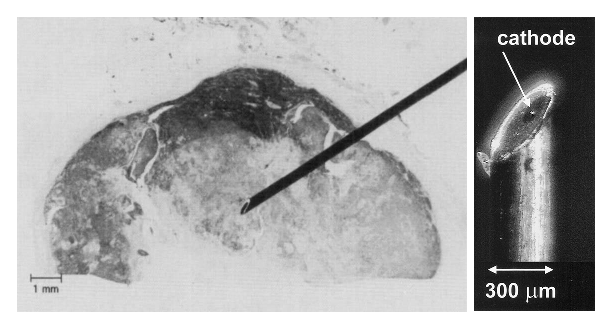
\includegraphics[scale = 1.2]{/Users/alex/Master/contents/images/eppendorf.eps}
\vspace{1cm}
\caption{(Left) Eppendorf polarographic needle electrode in a section of neck node metastasis taken from \textit{Nordsmark et al.}\cite{pmid8018370}. (Right) Close up of an Eppendorf electrode taken from \textit{Seddon et al.}\cite{pmid11352767}}
\label{fig:eppendorf}
\end{figure}
\subsection{Other methods for assessing hypoxia}\label{chap:otherhypoxiamethods}
In contrast to the above discussed approaches, \textit{Sovik et al.} \cite{pmid17674980} used dynamic contrast enhanced magnetic resonance (DCEMR) images to derive oxygen distribution. The distributions were created by inferring a direct proportionality of the time-averaged tracer concentration at a given point in the patient to the oxygen partial pressure in this region. The results were split into four compartments following the range of $p>20$ mmHg, $p=5-20$ mmHg, $p=[0.5-5]$ mmHg and $p = 0-0.5$ mmHg.
\section{Review of dose painting methods}
The deployment of PET has increased in the past years, mainly because PET has revolutionized imaging by giving radiation therapist a tool for anatomic localization of functional abnormalities in the complex territory of tumours. PET is used for staging, detection of unknown primaries and monitoring of treatment results. Dose painting is one the major concepts that involves the usage of PET to improve treatment planning. All dose painting approaches use a functional image such as PET or MRI to derive a dose escalation in one or the other way to account for hypoxic regions in tumour volumes. The way how the escalation is calculated can vary. Until now, dose painting by numbers (DPBN) has been used to prescribe a physical dose to hypoxic tumour volumes. The way how additional dose is prescribed to a clinical dose can be determined in various ways. This chapter will comment on all different dose painting methods used to overcome hypoxia.
\subsection{Binary dose escalation}
Binary dose escalation uses PET imaging to identify hypoxic tumours. If a lymph node or the primary tumour has a high tracer uptake value, it is considered to be hypoxic. The intensity of the imaging agent does not scale the additional boost that is administered in the this area. Therefore binary dose painting dose not incorporate any biological basis for the prescription. Multiple studies have been performed with this approach \cite{pmid20855118, pmid11240261, pmid17869020, pmid19203843}.\\One of the major findings derived from binary dose painting is that dose escalations can be achieved in most patients without compromising the dose limits to critical structures. Some cases were considered not the be feasible with this approach as they had critical organs (brainstem or spinal coord) very close to the target volumes \cite{pmid20855118}. In a study performed by \textit{Chao et al.} \cite{pmid11240261} using an Cu-ATSM imaging agent results showed feasibility of dose escalations in hypoxic sub volumes in head and neck cancer, without compromising OAR constraints. While the GTV was treated with a dose of 70 Gy, its hypoxic sub volume was treated with a dose of 80 Gy. Another study conducted by \textit{Lee et al.} \cite{pmid17869020} using FMISO guided IMRT found that dose escalations could easily be increased to 84 Gy (based upon a 70 Gy original prescription) and up to 105 Gy in one patient, without exceeding dose limits for critical structures. 
\subsection{Functional dose escalation}
Functional dose escalations use a prescription function to calculate dose escalations. The way how the functional image is interpreted and incorporated into the treatment planning process are quite different from their implementation.
\begin{itemize}
\item \textit{Cost function manipulations: }:  Rather than manipulating the dose prescription directly, this approach featured a dose efficiency $e(\vec x)\in[0,1]$, which was coupled with the dose-based cost function of the optimization algorithm to incorporate functional images such as PET. This way, the dose-based cost function $F(d(\vec x))$ was replaced with $F(d(\vec x)e(\vec x))$ instead. The analytical form of $e(\vec x)$ is very important since it will directly alter the way how the biological image will change the results of treatment planning. In a study performed by \textit{Alber et al.} \cite{pmid12587912} this function was rather simple as it represented a linear transformation of the signal intensity above a signal threshold
\begin{equation}\label{eq:alber}
e(\vec x) = 
\begin{cases}
\frac{1}{D_{\mathrm{Max}}}\left(D_{\mathrm{p}} +\frac{D_{\mathrm{max}}-D_{\mathrm{p}}}{I_{\mathrm{mean}}+I_{\mathrm{max}}}(i(\vec x)-I_{\mathrm{max}})\right) & I\geq I_{\mathrm{mean}}\\
1 & I< I_{\mathrm{mean}}.
\end{cases}
\end{equation}
Here $D_{\mathrm{Max}}$ is the maximum dose, $D_{\mathrm{p}}$ the prescribed dose, $I_{\mathrm{mean}}$ the mean intensity, $I_{\mathrm{max}}$  the maximum intensity of the functional image and $I(\vec x)$ the intensity at position $\vec x$. This simple prescription function is safeguarded against unreasonable dose escalations as it will use a linear prescription mechanism. On the downside, this functional prescription does not incorporate the underlying biology in a patient that can be acquired through PET.
\item \textit{Direct dose escalations: }Rather than manipulating the objective function in the treatment planning system to incorporate functional imaging it is possible to directly manipulate dose escalations. The magnitude of changes that are induced by such a dose escalation are dependent on the analytical form of the escalation function. Multiple studies have proposed different approaches to this problem. \textit{Bentzen et al.}\cite{pmid21356478} used a linear interpolation method
\begin{equation}\label{eq:bentzen}
D(I) = D_{\mathrm{Min}} + \frac{I-I_{\mathrm{Min}}}{I_{\mathrm{Max}}-I_{\mathrm{Min}}}\left(D_{\mathrm{Max}}-D_{\mathrm{Min}}\right).
\end{equation}
The dose escalation method proposed in equation \ref{eq:bentzen} has also been used in an adaptive dose painting study performed by \textit{Duprez et al.} \cite{pmid20643512} to create an FDG PET intensity based voxel-specific dose painting and has shown promising results in terms of feasibility. In a corresponding study, \textit{Madani et al.} \cite{pmid21742392} determined the maximum tolerated dose (MTD) in a phase I trial with 21 patients. The escalated median dose was elevated up to 80.9 Gy in the CTV and 85.9 Gy in the GTV. All surviving patients did not show any grade $\geq 4$ toxicity (life threatening or disabling side-effects) during treatment and follow-up, with the exception of mucosal ulcers. \\In general equation \ref{eq:bentzen} and equation \ref{eq:alber} use the same kind of linear transformation to incorporate functional imaging into the optimization process. Nevertheless, the level of impact can be quite different, as the latter directly manipulates the optimization process in the objective function, while \textit{Bentzen et al.} use dose scaling. \textit{Flynn et al.} \cite{pmid18635895} used a slightly different formula, which incorporated a linear scaling to dose boost $D_{\mathrm{Boost}}$ added on top of the original dose prescription $D_\mathrm{CTV}$ in the clinical target volume
\begin{equation}
D(I) = D_\mathrm{CTV} + \frac{I}{I_\mathrm{Mean}}D_\mathrm{Boost}.
\end{equation}
\end{itemize}
Physical dose painting that relies on a direct functional interpretation of the PET intensity, does not incorporate any considerations for the underlying biology. Therefore dose escalations are arbitrary as well as dependent on the functional form of the prescription function. \textit{Bowen et al.} \cite{pmid19218733} performed a study on the sensitivity of IMRT dose optimization to the mathematical form of a biological imaging-based prescription function. Polynomial functions were tested to simulate a continuous prescription, while sigmoidal functions were used to account for a threshold scenario. In addition two concepts were checked with both functions:
\begin{enumerate}
\item Prescribe a constant integral dose in the primary tumor volume.
\item Prescribe a maximum boosted dose to the primary tumour volume without fulfilling any integral dose constraints.
\end{enumerate}
\paragraph{Polynomial functions: }In general, polynomial functions represent a continuous prescription scenario. Depending on the exponent in the polynomial, the behaviour of prescription may change in different situations. A dose distribution planned using a square root function most closely resembles its prescription due to the smoothing of the dose gradients at higher dose boosts and the tighter distribution of prescribed dose about its mean. Square root functions therefore prescribe lower dose escalations to larger fractions of the PTV. On the other hand, a dose distribution resulting from the use of a quadratic prescription function least resembles its prescription due to the sharpening of these same dose gradients at higher dose boosts and larger spread in the distribution of prescribed dose about its mean. Quadratic prescription functions prescribe a higher dose to a smaller volume fraction. Therefore it becomes more and more difficult to deliver conformal dose distributions as the boost volumes become smaller in comparison to the treatment volume \cite{pmid17921573}.
\paragraph{Sigmoidal functions: }This function type is compatible with a threshold scenario. Sigmoidal functions are shaped with two parameters: slope and threshold position. Both parameters are not independent of each other, as changes in dose delivery are dependent on alterations in slope and the position of the threshold.  Increasing the prescription sigmoid slope at low threshold position yields to boosting of an increasing volumetric fraction of the PTV, while imposing steep gradients at the edges. Shifting the threshold towards a more central position, the dependence on the prescription slope becomes significant. Each voxel is equally sensitive to the steeper dose gradients, which causes smearing of the delivered dose as well as severe overdosed and underdosed regions \cite{pmid17921573}. 
\subsection{Dose painting by numbers via kinetic models}
Although most of the dose painting methods above can be categorized under the term 'dose painting by numbers', all of them lack the direct connection to a biological motivation for dose escalation. In a planning study by \textit{Thorwarth et al.} \cite{pmid17448882} hypoxia was incorporated into a new DPBN approach. Three plans were created to evaluate the outcome of DPBN: A conventional IMRT plan, a uniform dose escalation (binary dose painting) and hypoxia DPBN. The latter was nested into a planning framework by creating dose escalation factors (DEF) from a kinetic compartment model \cite{pmid15876662}. The model described the behaviour of FMISO trapped in hypoxic cells and its diffusion in interstitial space. This allows for a better identification of severely hypoxic and necrotic tissue than with SUV. DEFs were calculated with regard to local cell survival $M_i$ through a TCP model \cite{pmid16321146}
\begin{equation}
M_i = \exp\left(\frac{b\cdot \mathrm{TR}_i}{\mathrm{VP}_i+c}\right),
\end{equation}
where $\mathrm{TR}_i$ and $\mathrm{VP}_i$ are the tracer retention and vascularization-perfusion parameters for the $i$th voxel. The parameters $b$ and $c$ are acquired through the TCP model. Once the local cell survival $M_i$ is calculated, DEF can be calculated based on the mean radio sensitivity parameter of the linear quadratic model $\alpha$.
\begin{equation}
\mathrm{DEF}_i = \frac{\alpha D}{\alpha D - \ln M_i}.
\end{equation}
Here $D$ is the prescribed dose in the tumour volume. In the corresponding planning study, dose escalation was limited to 2.4 Gy per fraction, which was equal to DEF=1.2. DPBN via kinetic modelling assigns dose escalations of 2.2 Gy per fractions on small sub volumes that have a significantly higher survival due to hypoxia. DEF may vary on a larger scale from 1.03 up to 1.66, leading to problems with the limited dose of 2.4 Gy per fraction. This is mostly due to a combination of severe hypoxia and low vascularization and perfusion. This approach has been reevaluated in a later study by comparing predicted survival from the kinetic model with a FMISO PET image after 20 Gy direct evaluation \cite{pmid18524387}.
\subsection{Dose redistribution}
Rather than escalating the dose in hypoxic regions of the tumour, dose redistribution around a mean dose $D_\mathrm{mean}$ can be created by requiring
\begin{equation}
D_\mathrm{mean} - \sum\limits_{i=1}^NV_{ij}D_{ij} = 0,
\end{equation}
where $N$ is the number of compartments in the tumour, $V_{ij}$ the volume fraction of the compartment $i$ at treatment fraction $j$. A study by \textit{Sovik et al.} \cite{pmid17674980} applied IMRT to achieve the dose gradients needed from the guidance of the tumour map. It showed that IMRT dose distributions are less steep than the prescribed ones, as dose gradients are not completely  achievable with IMRT. This fact will become important for the approach that will be proposed in this thesis, as the same behaviour is shown. In the study, hypoxia compartments were derived with the approach described in chapter \ref{chap:otherhypoxiamethods}. Generally, dose in compartments with high pO2 values was too high, while compartments with lower pO2 values was to lower. The compartments that were assigned to oxygen partial pressure between 5 mmHg and 20 mmHg, approximately matched the prescriptions. The major drawback on this dose painting approaches is the application of a compartment model used to categorize hypoxia levels with their corresponding assignment of dose redistribution. \textit{South et al.} \cite{pmid19928068} investigated the relationship between the complexity of the dose prescription and the tumour control probability. The results show, that most heterogeneous biological distributions divided by a few dose levels compartments show the beneficial tumour control. However, this is only true, when the prescribed dose level and the compartment geometry is well chosen. Therefore, the usage of compartments might show unpredictable behaviour in contrast to a method that does not rely on the quantization of dose level compartments.
\subsection{Other approaches}
\section{Novel approach: biological dose painting}
Hypoxia reduces radio sensitivity and if it is not properly accounted for, leads to overestimation of cell kill for a given dose. With the help of the optimization of biological effect and incorporation of HRF into the model, it is possible to increase cell kill in hypoxic areas by an appropriate escalation of dose. This chapter introduces a novel approach of biological dose painting to achieve this.
\subsection{Implementation of biological dose painting in KonRad}
The first step in biological dose painting is to convert the SUV uptake values to oxygen partial pressure via equation \ref{eq:changmodel}. This oxygen partial pressure can then be transformed to a HRF for every voxel using equation \ref{eq:hrfmodel}. Afterwards, a prescribed biological effect is calculated based on the prescribed physical dose. In a third step, the optimization begins to use the quadratic biological function to find the best possible treatment plan with due regard to normal tissue constraints as well as the biological effect prescriptions. Within every optimization step, the delivered effect $\varepsilon_D$  is evaluated for every voxel. $\varepsilon_D$ is calculated with
\begin{equation}
\varepsilon_D = \frac{\alpha_X}{\mathrm{HRF}}D+\frac{\beta_X}{\mathrm{HRF}^2}D^2,
\end{equation}
where $D$ is the current dose in the voxel. The optimization stops if the relative value change of the biological optimization function is less than 0.01 during the last 6 optimization steps. The resulting physical dose distribution is analyzed to make plan comparisons simpler\\As seen in equation \ref{eq:dosecompensation}, the optimizer will compensate for hypoxia by scaling the dose linearly with the HRF. In most cases however normal tissue constraints will limit dose escalation in hypoxic volumes (cf. chapter \ref{chapter:4}).
\subsection{Clinical tumour hypoxia}\label{chap:tumourhypoxia}
In a meta-study by \textit{Jens Overgaard} \cite{pmid21511351} a total of 4805 patients with head and neck cancer were reviewed in terms of dose boosting in radiotherapy. In general, overall hypoxic modifications of radiotherapy will result in therapeutic benefits as it increases local regional control. This was also found to be independent of the type of modification used to circumvent the high radioresistance of hypoxic tumour areas. In order to estimate a realistic treatment environment for dose painting the first step is to evaluate Eppendorf polarographic needle measurements in head and neck cancer patients. A total of 551 patients have been found through comprehensive literature search. In most studies, pO2 values were separately measured in primary tumour volumes and lymph nodes. Every study presented in table \ref{tab:po2parameter} (if not noted otherwise) has conducted an evaluation of regions with pO2 $\leq 2.5$mmHg and $\leq 5.0$mmHg, as well as a mean pO2 value. In general primary tumours and lymph nodes do not seem to deviate in mean value or volume distributions of hypoxia. Therefore there should be no differentiation in treatment approaches for these two targets. The mean value pO2 value in head and neck cancer has been measured as $10.36 \pm 2.04$ mmHg. The hypoxia levels have been measured as $16.09 \pm 4.65$\% with $\leq 2.5$mmHg and  $36.38 \pm 6.80$\% with $\leq 5.0$mmHg. This shows that head and neck tumours are generally hypoxic and hold a small fraction of highly hypoxic cells, which could lead to failure of local tumour control. Likewise, the range of mean values and volume percentages measured can be very large. Therefore it is important to customize the treatment for every patient which requires a deeper understanding in the link between FMISO tracer uptake values and the underlying oxygen partial pressure (cf. chapter \ref{chap:hypoxiacorrelation}). One of the goal of this thesis is to proof feasibility of dose painting in head and neck cancer patients. Therefore, all patients presented in this work, will be treated as an average hypoxia patient. The following assumptions are made for all patients:
\begin{itemize}
\item Every patient investigated in this thesis is assumed to exhibit the same hypoxic properties. This means that model parameters used in this approach are the same for every patient.
\item Only the gross tumour volume (GTV) is hypoxic. All lymph nodes were considered to be normoxic.
\item The GTV exhibits a mean oxygen partial pressure of 10mmHg. The GTV contains two sub volumes consisting of hypoxic voxels with oxygen partial pressure of 5.0 mmHg and 2.5 mmHg (cf. chapter \ref{chap:tumourhypoxia} for detail construction of hypoxic volumes).
\end{itemize}
As patients are treated with radiation, the underlying biology changes. In terms of hypoxia, the biggest impact is associated with reoxygenation. The investigations of \textit{Lartigau et al.}\cite{pmid9797698} and \textit{Stadler et al.}\cite{pmid9783887} have shown that reoxygenation can clearly be measured after 32 Gy and 30 Gy of delivered dose respectively. In the study by \textit{Lartigau et al.} the mean oxygen partial pressure change up to 58\%, while the size of the highly hypoxic volume ($\leq 2.5$mmHg) shrunk from 14\% to 5\%. The same behaviour was observed in the measurements of \textit{Stadler et al.}. In primary tumour sites, the mean oxygen partial pressure increased up to 25\%, while the $\leq 2.5$mmHg and $\leq 5.0$mmHg volumes did not see any decrease. However, hypoxic volume reduction can be deduced by looking at the decreased statistical error on the volume measurements. 
\begin{sidewaystable}[p]
\centering
\small
\begin{tabular}{lccccc}
\toprule
\multicolumn{3}{c}{Study Information} & \multicolumn{3}{c}{pO2 Data [Range]}\\
\cmidrule(r){1-3} \cmidrule(r){4-6}
Study by & Type & Patients & Mean [mmHg] & $\leq$ 2.5 mmHg [\%] & $\leq$ 5.0 mmHg [\%]\\\\
\midrule\\
\textit{Becker et al.}\cite{pmid9765692}		& PT & 23 &  12.37 $\pm$ 10.18 [0.2-58.5] & 18.03 $\pm$ 22.54 [0.0-73.1] & 25.97 $\pm$ 38.64 [0.0-86.2]\\
									& LN & 22 &  13.71 $\pm$ 12.94 [1.9-50.3] & 18.56 $\pm$ 21.92 [0.0-66.0] & 27.86 $\pm$ 25.78 [0.0-88.5]\\
									& M & 30 &  43.78 $\pm$ 10.11 [20.8-67.7] & 0.36 $\pm$ 0.94 [0.0-5.1] & 0.95 $\pm$ 1.45 [0.0-7.6]\\\\
\textit{Lartigau et al.}\cite{pmid8453553}		& LN & 9 & 14.67 $\pm$ 11.86 [0.0-39.0] & 18.95 $\pm$ 30.04 [0.0-100.0] & -\\\\
\textit{Lartigau et al.}\cite{pmid9797698}		& C & 14 & 18.37 $\pm$ 12.81 [1.5-38.0] & 14.11 $\pm$ 18.02 [0.0-60.0]$^*$& -\\
									& C (32 Gy) & 14 & 28.92 $\pm$ 28.77 [3.0-100.0] &  4.89 $\pm$ 8.74 [0.0 - 30.0]$^*$& -\\\\
\textit{Nordsmark et al.}\cite{pmid16098619}	& C & 397 & 10.375 $\pm$ 3.57 [0.0-62.0] & 16.26 $\pm$ 9.01 [0.0-95.0] & 33.50 $\pm$ 14.24 [0.0-100.0]]\\\\
\textit{Stadler et al.}\cite{pmid9783887}		& PT & 2 & 7.50 $\pm$ 5.50 [2.0-13.0] & 25.50 $\pm$ 24.5 [1.0-50.0] & 38.50 $\pm$ 31.5 [7.0-70.0]\\
									& LN & 21 &  19.48 $\pm$ 15.33 [0.0-47.0] & 23.24 $\pm$ 20.47 [0.0-76.0] & 33.67 $\pm$ 26.68 [0.0-92.0]\\
									& PT (30 Gy) & 3 &  9.34 $\pm$ 3.40 [6.0-14.0] & 26.34 $\pm$ 12.12 [10.0-39.0] & 38.00 $\pm$ 9.89 [24.0-45.0]\\
									& LN (30 Gy) & 16 &  10.0 $\pm$ 11.13 [0.0-35.0] & 35.75 $\pm$ 23.38 [0.0-68.0] & 46.32 $\pm$ 22.90 [0.0-70.0]\\\\
\bottomrule\\
\textbf{Combined (PT)} & & 28 & 9.10 $\pm$ 2.79 [0.0-58.5] & 24.64 $\pm$ 9.79 [0.0-100.0] & 37.37 $\pm$ 9.17 [0.0-92.0]\\\\
\textbf{Combined (LN)} & & 68 & 12.77 $\pm$ 6.28 [0.0-50.3] & 24.38 $\pm$ 11.62 [0.0-76.0] & 37.37 $\pm$ 9.17 [0.0-100.0]\\\\
\bottomrule\\
\textbf{Combined (All)}$^\#$ & & 551 & 10.36 $\pm$ 2.04 [0.0-100.0] & 16.09 $\pm$ 4.65 [0.0-76.0] & 36.38 $\pm$ 6.80 [0.0-100.0]\\\\\\
\end{tabular}
\caption{pO2 values for different head and neck studies. All pO2 values were acquired with the help of Eppendorf polarographic needle measurements (if not stated otherwise). Errors are standard deviation of the given data and sample size. Combined data are gather through weight of standard deviation and number of patients screened. C = Combined (Tumor \& Nodes), LN = Lymphnodes, M = Muscle Tissue, PT = Primary Tumor. Remarks: $^*$ $\leq$ 2.0 mmHg, $^\#$ not including muscle tissue pO2 values}
\label{tab:po2parameter}
\end{sidewaystable}
\subsection{PET imaging}\label{chap:petimaging}
A comprehensive literature search has been conducted to evaluate the uptake values of FMISO and FDG tracers in head and neck cancer. In total 122 patients with FDG and FMISO images have been investigated. Most of the studies presented in table \ref{tab:suvparameter} have been able to examine the uptake values of FMISO and FDG. Tracer uptake was characterized by using the maximum and mean tissue radioactivity concentration $c_i(t)$ to derive SUV. In general FDG uptake is higher than FMISO. Mean FDG SUV have been measured as $SUV_\mathrm{mean}=3.75 \pm 0.24$, while maximum SUV is  $SUV_\mathrm{max}=9.63 \pm 1.1$. For FMISO these values can be quantified with $SUV_\mathrm{mean}=1.76 \pm 0.16$ and $SUV_\mathrm{max}=2.28 \pm 0.32$. The found results for PET images with FDG and FMISO are used to make the following assumptions for further investigations in this thesis:
\begin{itemize}
\item PET images will are assumed to represent FMISO and not FDG uptake distributions.
\item The maximum SUV = 2.28 was assigned to the highly hypoxic regions in head and neck cancer according to table \ref{tab:po2parameter}. Therefore, if the FMISO SUV is equal to 2.28, a 2.5 mmHg oxygen partial pressure is inferred in this voxel.
\item To incorporate the maximum SUV correlation to 2.5 mmHg hypoxia levels, the pO2 model from equation \ref{eq:changmodel} has to be modified to account for this assumption. This can be easily done by changing the $I_\mathrm{max}$ to its  appropriate value, such that an intensity of $I=2.28$ yields $p=2.5$ mmHg
\begin{equation}\label{eq:gaugedchang}
2.5\mathrm{mmHg} = 6.4\mathrm{mmHg}\left(\frac{I_\mathrm{max}}{2.28}-1\right) \rightarrow I_\mathrm{max} = 3.17 \pm 0.77.
\end{equation}
\end{itemize}
Just as with direct measurements of oxygen partial pressure, reoxygenation can be clearly seen in a study conducted by \textit{Eschmann et al.}\cite{pmid17543402}. It was found that the FMISO uptake after a total dose of 45 Gy decreased about 30\%, while the range of FMISO SUV change from 1.7-4.4 to 1.4-3.0. As lower FMISO retention is directly linked to higher oxygen partial pressure, it can be concluded that reoxygenation has occurred. By understanding the reoxygenation behaviour for a dose painting approach, treatment planning could be improved even further. Chapter \ref{chap:reoxygenation} will discuss the impact of reoxygenation and its impact on dose painting.
\begin{sidewaystable}[p]
\centering
\footnotesize
\begin{tabular}{lccccccc}
\toprule
\multicolumn{3}{c}{Study Information} & \multicolumn{2}{c}{FDG Uptake Data [Range]} & \multicolumn{2}{c}{FMISO Uptake Data [Range]}\\
\cmidrule(r){1-3} \cmidrule(r){4-5}\cmidrule(r){6-7}
Study by & Tracer(s) &Patients & Mean [SUV] & Maximum [SUV]& Mean [SUV] & Maximum [SUV]\\
\midrule\\
\textit{Eschmann et al.}\cite{pmid17543402}	& FMISO & 14 & - & - & 2.56 $\pm$ 0.75 [1.7-4.4] & -\\
									& FMISO (45 Gy) & 14 & - & - & 1.99 $\pm$ 0.44 [1.4-3.0] & -\\\\
\textit{Gagel et al.}\cite{pmid15480509}		& FMISO/FDG & 16 & 8.14 $\pm$ 3.58 [3.3-17.4] & 9.98 $\pm$ 4.60 [4.6-20.0] & 1.76 $\pm$ 0.37 [1.2-2.2] & 2.07 $\pm$ 0.4716 [1.4-3.0]\\\\
\textit{Komar et al.}\cite{pmid18997048}		& FDG & 13 & 6.14 $\pm$ 3.01 [2.6-14.1]$^\&$ & 8.94 $\pm$ 4.49 [4.2-22.1]$^\&$ & - & -\\
									&  & 5 & 6.14 $\pm$ 3.01 [2.6-14.1]$^\#$ & 6.33 $\pm$ 1.78 [4.2-8.5]$^\#$ & - & -\\\\
\textit{Lehti\"o et al.}\cite{pmid15234030}		& FDG & 20 & 13.07 $\pm$ 5.76 [5.3-28.8]$^*$ & - & - & -\\
									&  & 7 & 9.70 $\pm$ 3.64 [5.7-16.2]$^\#$ & - & - & -\\
									&  & 7 & 11.94 $\pm$ 3.14 [7.2-19.0]$^\&$ & - & - & -\\\\
\textit{Nehmeh et al.}\cite{pmid18086391}	& FMISO/FDG & 14 & 34.1 & 28.70 $\pm$ 38.36 [7.3-136.6] & 2.9 & 2.86 $\pm$ 0.63 [1.9-4.5]\\\\
\textit{Thorwarth et al.}\cite{pmid16920211}	& FMISO/FDG & 12 & 3.39 $\pm$ 0.24 [3.0-3.9] & 9.38 $\pm$ 1.16 [7.9-12.1] & 1.22 $\pm$ 0.19 [0.9-1.5] & 2.09 $\pm$ 0.59 [1.4-3.2]\\\\

\bottomrule\\
\textbf{Combined} & & 122 & 3.75 $\pm$ 0.24 [2.6-34.1]& 9.63 $\pm$ 1.10 [4.2-136.6] & 1.78 $\pm$ 0.16 [0.9-4.4] & 2.28 $\pm$ 0.32 [1.4-4.5]\\\\\\
\end{tabular}
\caption{Uptake values for FMISO and FDG PET images from different head and neck studies. Errors are standard deviation from data withhin corresponding study. Remarks: $^*$ Combined SUV uptake (Primary Tumor Volume \& Lymphnodes), $^\#$ Metastasis/Lymph Nodes, $^\&$ Primary Tumor.}.
\label{tab:suvparameter}
\end{sidewaystable}
\section{Implementation of biological dose painting}\label{chapt:clinicalimplementation}
The implementation of biological dose painting uses all assumptions made in chapter \ref{chap:tumourhypoxia} and \ref{chap:petimaging}. One of the most important assumptions in this regard, is the way how hypoxia is modelled in head and neck patients. This chapter will deal with the clinical implementation of hypoxia in head and neck cancer as well as methods to compare clinically approved plans to biologically dose painted plans.
\subsection{Creation of realistic artificial PET images}
\begin{table}[b]
\centering
\small
\begin{tabular}{ccc}
\toprule
pO2 (VOI) & HRF & Clinical \% of GTV\\
\midrule\\
$\leq$ 2.5 mmHg (GTV$_{2.5}$) & 1.80 $\pm$ 0.04 & 16.09 $\pm$ 4.65\\\\
$\leq$ 5.0 mmHg (GTV$_{5.0}$) & 1.51 $\pm$ 0.03 & 36.38 $\pm$ 6.80\\\\
$\approx$ 10.0 mmHg (GTV)& 1.30 $\pm$ 0.01 & 100\\\\
\bottomrule\\
\end{tabular}
\caption{HRF values for different hypoxic regions in head and neck patients. Parameters for calculations for HRF$_0$ are $m$ = 2.82 $\pm$ 0.05 and $K$ = 1.94 $\pm$ 0.13 mmHg. Errors were calculated using the Gaussian error propagation method.}
\label{tab:HRFparameters}
\end{table}
No FMISO images were available for the 10 patients in this study. Therefore, artificial PET images were generated for this thesis. A small software was written to generate PET images based on the patients volumes of interest. \textit{PETCreate3} is a fast C-based PET image generator coupled with a point-in-polygon (PIP) algorithm. A number of PIP algorithms has been developed after its early description in 1974 \cite{Sutherland}. \textit{PETCreate3} uses a winding number algorithm, which utilizes the fact that the sum of all angles formed by the point of interest with the constituent points of a polygon will add up to multiples of 2$\pi$, if the considered point lies within the polygon.\\The construction of hypoxic volumes is based on the GTV for all patients. The GTV was assumed to be hypoxic with  pO2 = 10 mmHg. Smaller hypoxic sub volumes representing the 5.0 mmHg and 2.5 mmHg hypoxia levels were created by applying negative safety margins to the GTV. The volumes were created with the virtual treatment planning software \textit{VIRTUOS}. As GTVs can differ in size and form, the accuracy of this construction mechanism can fluctuate, as the smallest applicable safety margin in \textit{VIRTUOS} is 1 mm.\\The general goal of this approach was to create volumes with properties shown in table \ref{tab:HRFparameters}. According ti the pO2 model, the oxygen partial pressure of 2.5 mmHg and 5.0 mmHg represent specific HRF values, which can also be seen in table \ref{tab:HRFparameters}. In order to achieve the same biological effect as a prescribed dose of 70 Gy to an oxic volume, a dose $D = 126$ Gy has to be delivered if this volume has an oxygen partial pressure of 2.5 mmHg. In contrast to other dose painting approaches, biological dose painting can derive this dose from a model that has been realigned with clinical data.
\subsection{Plan comparison}\label{chap:plancomparison}
In radiotherapy, different treatment plans are frequently evaluated by comparing the dose distributions using dose volume histograms. In biological dose painting, the biological effect is more important than the physical dose. This thesis proposes using biological effect volume histograms (eDVH) to compare different plans. As seen in previous chapters, hypoxia and their derived HRF distributions will change the resulting optimized dose distributions and therefore the eDVH as well. However a direct comparison of the biologically dose painted plan with a nominal biological optimization is not feasible, as the latter assumes a fully oxic tumour volume. If such a comparison is made, the new approach will always be disadvantageous with respect to a normal biological optimization. Therefore such a nominal biological optimization has to be evaluated on the underlying biological tumour maps derived with the biological dose painting. The delivered biological effect for a nominal biological optimization evaluated on a hypoxia map is then
\begin{equation}
\varepsilon = \alpha_\mathrm{H} D + \beta_\mathrm{H}D^2,
\end{equation}
where $\alpha_\mathrm{H}$ and $\beta_\mathrm{H}$ are the hypoxic radio response parameters (decreased by HRF) and $D$ is the delivered dose of the nominal biological plan. As hypoxic volumes were constructed in the GTV, the eDVHs were only generated in the GTV (and therefore in the respective sub volumes GTV$_\mathrm{5.0}$ and GTV$_\mathrm{2.5}$). By applying this approach, a comparison was performed between the three plans:
\begin{itemize}
\item Biological dose painted plan on the hypoxia map derived from a FMISO PET image (plan 1)
\item Biologically optimized plan without the use of a PET image (plan 2). All dose distributions from this plan are evaluated on the hypoxia map which was used in plan 1 to assess the impact of hypoxia on delivered clinical plan.
\item Nominal biologically optimized plan, assuming a fully oxygenated tumour environment.
\end{itemize}

\chapter{Feasibility of Biological Dose Painting}\label{chapter:4}
% chapter 4: feasibility of dose painting

\section{Patients}
All patients presented in this work were diagnosed with head and neck cancer. Head and neck cancer has been identified as the sixth most common cancer worldwide \cite{pmid15685196}. Head and neck cancer can be categorized into five groups, named after the regions, where the cancer usually originates from: Laryngeal and hypopharyngeal cancer, nasal cavity and paranasal sinus cancer, nasopharyngeal cancer, oral and oropharyngeal cancer, salivary gland cancer \cite{Brockenstein}.\\The patients presented in this thesis have been diagnosed with oropharyngeal cancer. Access to treatment plan data for ten patients have been approved by the local Research Ethics Board of the Princess Margaret Hospital (Toronto, Ontario, Canada) for this dose painting study. Patients were originally treated with 70 Gy in 35 fractions and had a clinically approved plan available for direct comparison with plans generated with biological dose painting. Original treatment plans were generated with the \textit{Pinnacle 3} treatment planning system (Philips Radiation Oncology Systems, Fitchburg, Wisconsin, USA).
\section{Application of Biological Dose Painting}
Biological dose painting has been applied to the above described patients. In a first step, the provided patients were imported into the virtual treatment planning software \textit{VIRTUOS}. \textit{VIRTUOS} transform clinical plans to a format that can be imported to \textit{KonRad}. In a second step clinical target volumes were edited with the hypoxic sub volume construction based on the GTV (cf. chapter \ref{chapt:clinicalimplementation}). As the geometry of every patient is different and the accuracy of the negative safety margin applied to create the sub volumes is 1 mm, it is not always possible to achieve the same sizes. Afterwards patients undergo the following procedure to create plans with biological dose painting.
\begin{enumerate}
\item Create a nominal treatment plan with \textit{KonRad} until an adjust plan constraints with the \textit{Pinnacle} plan. Plan quality was assessed by target volume coverage and sparing of organs at risk. The nominal plan is created with a biological optimization without a PET image. The critical organ dose limits for both plans were based on the HN06 trial criteria \cite{HN06}. Afterwards, the treatment plan is approved by an experienced clinical medical physicist.
\item Application of biological dose painting to create a nominal dose painted plan. Due to the additional dose delivered into the hypoxic volumes in the GTV, iso-toxic treatment planning becomes more difficult. In most cases, dose limits in OARs can be achieved by changing overlap priorities in \textit{KonRad} to achieve a better treatment of critical structures. If dose painted plans were within limits of the HN06 trial or the clinically approved plan, they were again evaluated by a medical physicist or a physician.
\item Comparison between the approved nominal and biological dose painted plans created with \textit{KonRad}. A detailed description of methods used to compare the different results are presented in chapter \ref{chap:plancomparison}.
\end{enumerate}
All treated patients are listed in table \ref{tab:patientgtv}. The nominal plan created in \textit{KonRad} is based on the clinical plan generated with \textit{Pinnacle}. The latter is approved by an experienced clinical medical physicist and fulfills the dose limits of the HN06 clinical trial \cite{HN06}. The first goal was to achieve an equally good or better plan with a biological optimization without a PET image in \textit{KonRad}. All dose statistics for OAR and tumour volumes are attached in Appendix \ref{appendix:b}, as the nomenclature and number of incorporated treatment  volumes varies with every patient.
\begin{sidewaystable}[p]
\centering
\footnotesize
\begin{tabular}{cccccccccc}
\toprule
\multicolumn{2}{c}{Patient Information} & \multicolumn{2}{c}{Hypoxic volumes} & \multicolumn{2}{c}{Clinical plan dose [Gy]} &  \multicolumn{4}{c}{Biological dose painting [Gy]}\\
\cmidrule(r){1-2} \cmidrule(r){3-4}\cmidrule(r){5-6}\cmidrule(r){7-10}
Patient No & GTV volume [ccm] & GTV$_{5.0}$ [ccm]& GTV$_{2.5}$ [ccm] & $\overline D_\mathrm{GTV}$ & $D_\mathrm{GTV}^\mathrm{max} $ & $D_\mathrm{max}$ (GTV) &  $\overline D$ (GTV) & $D$ (GTV$_{5.0}$) & $D$ (GTV$_{2.5}$)\\
\midrule\\
1	&	124846	&	43380 (34.8\%)	&	11698 (9.4\%)	&	68.94	&	78.49	&	119.8	&	93.4	&	95.5	&	92	\\\\
2	&	8689	&	2858 (32.9\%)	&	-	&	72.19	&	76.32	&	88.3	&	81.9	&	84.3	&	-	\\\\
3	&	70948	&	31163 (43.9\%)	&	7805 (11.0\%)	&	71.13	&	76.47	&	120.9	&	88.9	&	94.4	&	104.6	\\\\
4	&	62626	&	24287 (38.8\%)	&	3389 (5.4\%)	&	71.39	&	76.78	&	112.5	&	80	&	86	&	96.8	\\\\
5	&	33984	&	13.831 (40.7\%)	&	3380 (10.0\%)	&	69.81	&	77	&	116.6	&	85.5	&	91.2	&	100.7	\\\\
6	&	127365	&	39528 (31.0\%)	&	9278 (7.3\%)	&	63.5	&	77.03	&	116.5	&	86.9	&	93.4	&	102.8	\\\\
7	&	42119	&	12231(29.0\%)	&	3902 (9.3\%)	&	71.58	&	78.26	&		&		&		&		\\\\
8	&	11342 (CTV70)	&	3939 (34.7\%)	&	702 (6.2\%)	&	71.54	&	75.91	&		&		&		&		\\\\
\bottomrule\\
\end{tabular}
\caption{Patient information columns show patient ID as well as the size of the treated GTV in ccm. Hypoxic volume column sizes of GTV$_{5.0}$ and GTV$_{2.5}$ are based on the GTV (=100\%). The guidance values for the hypoxic sub volume construction are GTV$_{2.5}=16.08\pm 4.65$ and GTV$_{5.0}=36.38\pm 6.80$. Clinical plan columns show the mean dose and maximum dose in the GTV. Biological dose painting columns show the theoretical dose values for equal biological effect due to HRF. HRF values are HRF$_{2.5}=1.8$ (GTV$_{2.5}$), HRF$_{5.0}=1.51$ (GTV$_{5.0}$) and HRF$_{10.0}=1.3$ (GTV).}
\label{tab:patientgtv}
\end{sidewaystable}
\section{Results}
\subsection{Impact of Hypoxia Sub Volumes in GTV}
As dose escalations were applied to the plan, critical structures need to be reevaluated with due regards to their dose limits set by the HN06 trial. The dose in hypoxic volumes is scaled linearly with HRF (cf. equation \ref{eq:dosecompensation}). For severely hypoxic voxels with less than 2.5 mmHg oxygen partial pressure HRF$_{2.5}=1.8$ and for hypoxic volumes with less than 5.0 mmHg HRF$_{5.0}=1.51$. The GTV itself has been shown to be hypoxic with an average of 10 mmHg (cf. table \ref{tab:po2parameter}). Therefore, the GTV is assigned to a value of HRF$_\mathrm{10}=1.3$. As the GTV size varies from patient to patient, the impact of biological dose painting can also vary. Patient 2 had a very small GTV, which did not allow the generation of a GTV$_{2.5}$ as it only encompassed about 100 voxels. Therefore dose escalations in this patient were smaller than in patients that have both sub volumes available for treatment planning. Patient 8 did not have a GTV as the tumour size had been surgically reduced. In this case, the CTV$_{70}$ has been used to create the hypoxic sub volumes. Table \ref{tab:patientgtv} shows all patients treated with the new approach of biological dose painting. Figure \ref{fig:DVH} shows a direct comparison of the GTV of the clinical plan with the GTV and hypoxic sub volumes of the dose painted plan. 
\begin{sidewaysfigure}[p]
\centering
\rotatebox{-90}{\includegraphics[scale = 0.8]{/Users/alex/Master/contents/images/DVH.eps}}
\caption{Dose volume histograms for the GTV of the clinical plan (green) and all volumes from biological dose painting: GTV (red), GTV$_{5.0}$ (blue), GTV$_{2.5}$ (magenta). Patient 2 did not have a GTV$_{2.5}$ as the GTV was to small. Complete delivery is not possible to the GTV and hypoxic sub volumes. Desired dose values are $D_{2.5} = 126$ Gy for the 2.5 mmHg sub volume, $D_{5.0} = 105.7$ Gy for the 5.0 mmHg sub volume and $D_\mathrm{GTV} = 91$ Gy for the GTV which was assigned with 10 mmHg.}
\label{fig:DVH}
\end{sidewaysfigure}
\subsection{Delivery Quality and Feasibility of Dose Painting}The general limitation of biological dose painting is set by the critical structures, which is also dependent on the geometry and size of the GTV itself. The overriding guideline for all biologically dose painted patients was the iso-toxic treatment of critical structures. This means that none of them were allowed to exhibit a larger maximum dose than in the clinical plan. If the clinical plan did not fully fulfill the HN06 trial dose constraints, while the biological dose painted plan did, it is still counted as an iso-toxic treatment. Table \ref{tab:patientgtv} shows the mean and maximum dose values for the GTV and its hypoxic sub volumes. The critical structures that limit the complete delivery of dose painting to the patient include the esophagus, parotids, mandible, larynx, spinal cord and the neck region. The latter usually exhibited a larger overlap with treatment volumes. Therefore those were omitted in the evaluation of the iso-toxic treatment. The limiting nature of these volumes stems from the fact that most clinical dose constraints in these volumes were below 70 Gy. As soon as dose painting is applied, higher dose up to 126 Gy (in the GTV$_{2.5}$) were considered in the optimization process. In most cases the GTV overlaps with critical structures, which leads to the high dose that does not comply to the iso-toxic treatment. Therefore overlap priorities have to be changed to guide the optimization to achieve the target dose constraints.\\Very good coverage was achieved in the GTV$_{5.0}$, while the GTV$_{2.5}$ suffer from cold spots in some cases. This is mainly because the GTV$_{2.5}$ is particularly small in comparison to the GTV and GTV$_{5.0}$, which requires large dose gradients to achieve the desired dose. Generally speaking, the maximum desired dose can not be achieved in most cases, as critical structures will limit complete delivery.\\Figure \ref{fig:R} shows the ratio $R$ of delivered biological effect to prescribed biological effect in the GTV (and hypoxic sub volumes). 
\begin{equation}
R = \frac{\varepsilon_\mathrm{delivered}}{\varepsilon_\mathrm{prescribed}}
\end{equation}
If $R=1$, the delivered effect is equal to the prescribed effect, while $R>1$ implies an over delivery and $R<1$ implies under delivery of biological effect in those voxels. The general form of the $R$ distribution does not change significantly in most patients. The $R$ value for patient 1 is shifter more to 1, while patient 4 shows a larger discrepancy for the dose painted plan. This is mainly due to the fact that patient 4 had larger overlap with the right neck volumes and the GTV which limited the dose delivery.
\begin{sidewaysfigure}[p]
\centering
\rotatebox{-90}{\includegraphics[scale = 0.8]{/Users/alex/Master/contents/images/R.eps}}
\caption{Ratio $R$ of delivered biological effect in the GTV divided by the prescribed effect. If $R>1$, the voxel is over dose, while $R<1$ can be interpreted as under dose. $R$ distributions show clinical plan (green) and dose painted plan (red). There are no significant changes in desired biological effect delivery. Patient 4 shows a slight change as the neck volumes had a larger overlap with the GTV.}
\label{fig:R}
\end{sidewaysfigure}
Generally feasibility of dose painting is only limited by critical structures in the way of the beam toward the GTV and hypoxic sub volumes. The maximum dose point is never achieved due to these limitations, which means that certain voxels were not treated adequately, while voxels that were in line with the beam and the GTV$_{2.5}$ will receive a higher dose. Critical structures limiting the feasibility of dose painting, depend on the size and shape of the GTV itself.
\subsection{Nominal Plan vs Biological Dose Painting}
To compare the effectiveness of biological dose painting to approved clinical plans, this thesis uses biological effect volume histograms (eDVH). The way, how eDVH were derived has been described in chapter \ref{chap:plancomparison}. Figure \ref{fig:eDVH} shows a direct comparison of a biological dose painted plan and a clinical plan in the GTV for all patients treated with dose painting. The clinical plan does not incorporate the underlying hypoxic effect of radioresistance in the GTV, which leads to an overestimation of cell kill. The delivered plan from the combination of the underlying tumour hypoxia and the clinical dose delivered into the GTV. Generally, the mean biological effect of planned clinical and dose painted plans were almost equal. This is due to the fact that dose painting compensates for the hypoxia present in the GTV. However, the quality of dose painted plans decreases, as the dose gradients become higher. This is especially reflected in the flattening of eDVH around the mean value for dose painted plans. Delivered plans eDVHs were derived from the combination of hypoxia maps and delivered dose from the clinical plan. This represents the biological effect achieved, if hypoxia is incorporated. The biological effect in delivered plans is always lower as the HRF decreases the mean delivered effect. The difference between the clinical plan the delivered plan in the eDVH in figure \ref{fig:eDVH} shows the reason for local failure in head and neck cancer, as cell kill is overestimated as hypoxia is not incorporated in the planning process.
\begin{sidewaysfigure}[p]
\centering
\rotatebox{-90}{\includegraphics[scale = 0.8]{/Users/alex/Master/contents/images/eDVH.eps}}
\caption{eDVH of GTV for all treated patients with biological dose painting. The biological effect of the delivered plan (blue) reduced through hypoxia is based on the clinical plan (green). Dose painting (red) is able to compensate for hypoxia by increasing the dose to such volumes. The dip in the eDVH for the delivered plan (blue) stems from the 2.5 mmHg hypoxia level.}
\label{fig:eDVH}
\end{sidewaysfigure}
\section{Discussion}
\subsection{Feasibility of Biological Dose Painting}
This work shows that biological dose painting is feasible while simultaneously conforming to dose constraints from an approved clinical plan. The implemented dose painting approach compensates for hypoxia derived from PET FMISO images by increasing the dose in such hypoxic volumes. In contrast to the delivered plan (derived from the hypoxia distribution from the PET image and the clinical plan), is able to achieve desired tumour control while sparing the OAR just as in the clinical plan. All plans did not achieve the anticipated maximum dose of 126 Gy based on the 70 Gy prescription of the clinical plan. This is mainly due to the following facts:
\begin{itemize}
\item The smallest hypoxic sub volume representing the 2.5 mmHg oxygen partial pressure is too small to generate the high dose gradients needed to achieve such a high dose points.
\item There are OARs in the way from the incident beam to the hypoxic volumes. The constraints on the OAR will decrease the maximum deliverable dose to the hypoxic sub volumes.
\end{itemize} 
The achieved biological effects with biological dose painting suffer from limitations from the organs at risk in the vicinity of the GTV and in between the incident beam and the hypoxic sub volumes. This leads to the flattening of the eDVH distribution, or in other words, a larger spread of biological effect when compared to the clinical plan without any hypoxia considerations. In comparison to the delivered plan, derived from the clinical plan, biological dose painting performs better than any conventional radiotherapy. The success of treatment in head and neck can be improved if dose painting is used clinically. This implies a better understanding of the functional imaging modality that is used to derive hypoxia. If the underlying tumour hypoxia derived from such an image is a realistic representation of the true pO2 distribution in a tumour volume, then dose painting could yield even better results. Chapter \ref{chapter:6} takes a closer look on how this can be incorporated into the current treatment planning framework.\\The flattening of eDVH distributions for biological dose painting can also be attributed to the construction of artificial PET images. As the intensities in the sub volumes are step functions, the treatment planning system try to create high dose gradients which can usually be never achieved in such a small region. In comparison to real PET images with FMISO, the artificial PET images are an extreme case. Usually FMISO distributions are smooth or in form of a blob within the hypoxic tumour volume. The gradual increasing intensity of tracer retention leads a smoother dose gradient which can be satisfied by the optimizer in an easier fashion. Therefore the delivery efficiency with biological dose painting can be increased when real PET images are used to start treatment planning.
\subsection{High Dose Fractions}
The biological model deployed in this work invoke a dose above 100 Gy. Usually radiotherapy rarely surpasses this dose value. If the implications of the biological model are correct, then 126 Gy are needed to overcome the highly hypoxic regions of the tumour to achieve local tumour control. The problem that arises from such high dose values is the damage done in the tumour volume itself, as it generally disintegrates all tissue types. In a treatment plan with 30 fractions a dose of 4.2 Gy is needed to achieve such a high dose in the hypoxic sub volumes. This of course is not feasible as the skin becomes highly irritated and should be avoided for the sake of patient's wellbeing. Rather than delivering such a high dose plan in 30 fractions, it could be feasible to achieve biological dose painting in 35-45 fractions as the fraction dose is within acceptable limits.
\subsection{Size of Hypoxic Volumes}
Depending on the size of the GTV, the hypoxic volumes generated with the approach used in this work get smaller than feasible for general dose delivery. This is mainly due to the fact that the steps from the GTV$_{5.0}$ to the GTV$_{2.5}$ theoretically dose increase from 105 Gy to 126 Gy. If the hypoxic sub volume is too small, such dose gradients cannot be generated with normal photon delivery, while an approach with protons or carbon ions could yield a much better result. The size of the small hypoxic volumes can also be problematic while positioning the patient while the treatment. Small errors in positioning can lead to a larger dose in parts of the tumour that are less hypoxic, while the highly hypoxic volumes receive a smaller dose. 
\section{Conclusion}
Biological dose painting is feasible for head and neck patients while conforming to clinical dose constraints. Dose escalations can be generated from a PET FMISO image and implemented into a treatment planning framework that accounts for hypoxia derived from a tumour map. Dose delivery does not completely achieve the desired maximum dose, but the biological effect delivered with biological dose painting compensated for hypoxia. The comparison with clinical plans show, that biological dose painting shows a huge advantage in treatment planning. The high dose needed to deliver dose painted plans should be split into more fractions to avoid complications with skin irritation and improve the wellbeing of the patient during treatment.

\chapter[Analysis of model parameter uncertainties]{Analysis of model parameter uncertainties on biological dose painting}\label{chapter:5}
% chapter 5: efficacy of dose painting on uncertain radiobiological tumor maps
The biological model deployed in this novel approach to dose painting encompasses four different parameters. While the $I_\mathrm{max}$ is a parameter that is dependent on the tracer (here FMISO) and has to be adapted to clinical oxygen values from direct Eppendorf measurements. A robustness analysis was performed for biological dose painting to assess the impact of model uncertainties. For this, the approved biological dose painted plan on the mean model parameters was used to evaluate changes of biological effect on new tumour maps derived from model parameter combinations. Three parameters were evaluated within their standard deviation, which means that every parameters had a lower limit (mean - standard deviation), mean and upper limit (mean + standard deviation). Therefore, $3^3=27$ plans have to be evaluated by comparing the eDVH distributions and their impact on the delivered effect from their underlying HRF distributions. 
\section{Model parameter uncertainties}
This work will investigate all parameters involved in the calculation of dose escalation factors in hypoxic sub volumes. The theoretical implications of the errors on the model parameters $p_{50}$, $K$ and $m$ are shown in figure \ref{fig:uncertaintyimpact}. The largest deviation in HRF transformation is given by the $p_{50}$ parameters, while $m$ and $K$ have a smaller impact. 
\begin{figure}[p]
\centering
\subfigure[$K=1.81$ mmHg, $m=2.77$]{
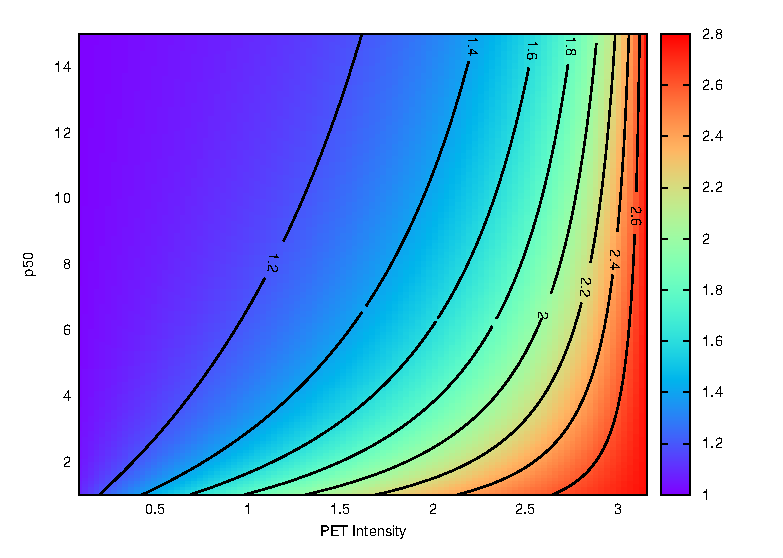
\includegraphics[scale = 0.525]{/Users/alex/Master/contents/images/K181m277.eps}
}
\hspace{0.3cm}
\subfigure[$K=2.07$ mmHg, $m=2.87$]{
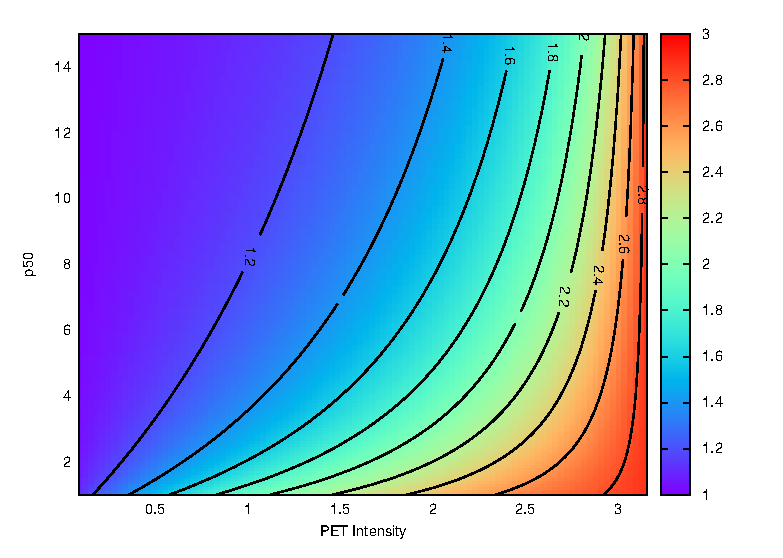
\includegraphics[scale = 0.525]{/Users/alex/Master/contents/images/K207m287.eps}
}
\hspace{0.3cm}
\subfigure[$K=1.81$ mmHg, $p_{50}=1$ mmHg]{
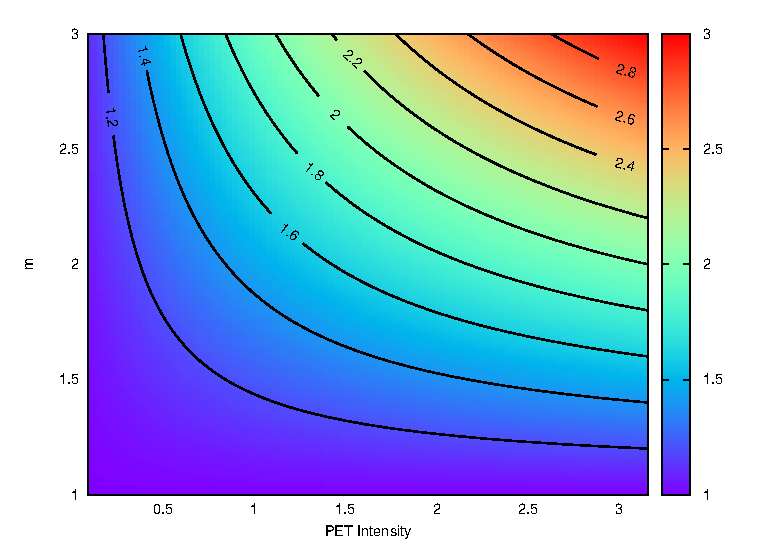
\includegraphics[scale = 0.525]{/Users/alex/Master/contents/images/K181p1.eps}
}
\hspace{0.3cm}
\subfigure[$K=2.07$ mmHg, $p_{50}=11.8$ mmHg]{
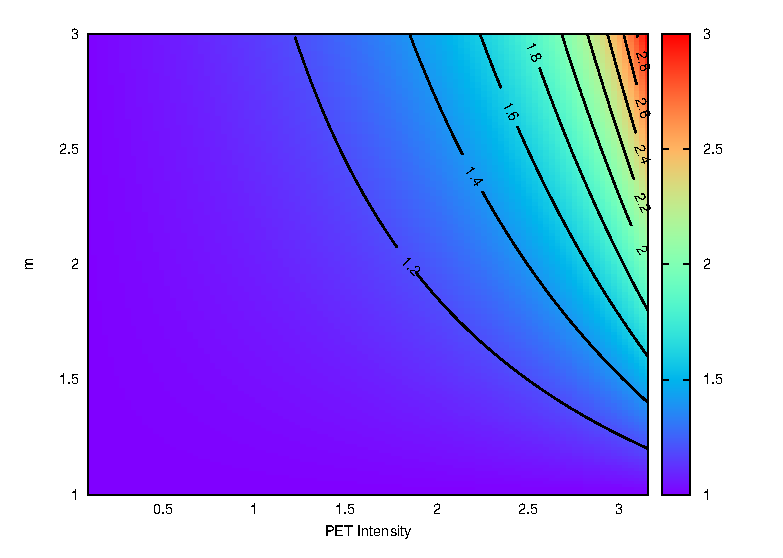
\includegraphics[scale = 0.525]{/Users/alex/Master/contents/images/K207p118.eps}
}
\subfigure[$m=2.77$ mmHg, $p_{50}=11.8$ mmHg]{
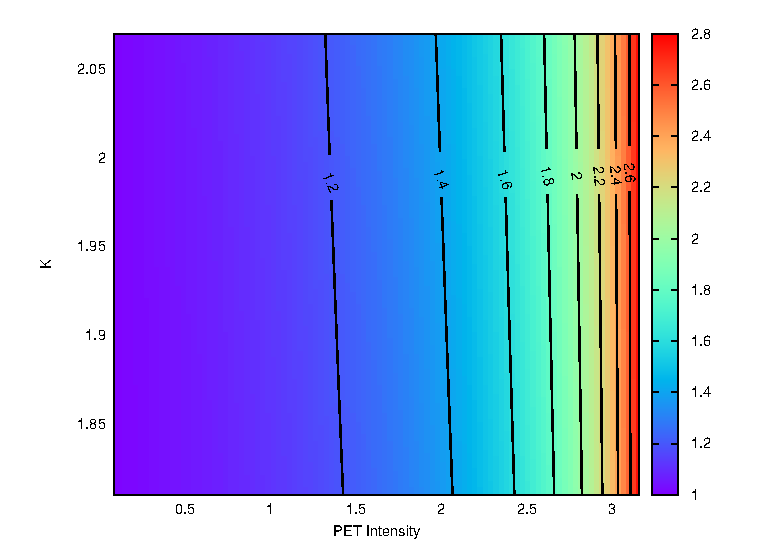
\includegraphics[scale = 0.525]{/Users/alex/Master/contents/images/m277p118.eps}
}
\hspace{0.3cm}
\subfigure[$m=2.87$ mmHg, $p_{50}=1$ mmHg]{
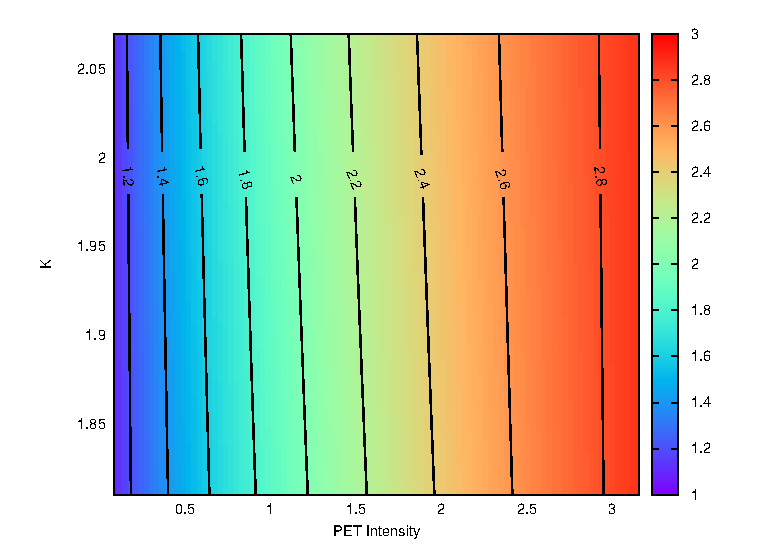
\includegraphics[scale = 0.525]{/Users/alex/Master/contents/images/m287p1.eps}
}
\caption{Impact of model uncertainties on the HRF derived from the signal of a PET FMISO image in the SUV range of 0 up to 3.17. The lowest impact on the HRF prescriptions is seen with $K$, while $p_{50}$ and $m$ introduces the largest HRF changes in the transformation model.}
\label{fig:uncertaintyimpact}
\end{figure}
\subsection{pO2 model}
The pO2 model from \textit{Chang et al.} uses two parameters. The $I_\mathrm{max}$ parameters is a parameters, which can be adjusted to the latest pO2 measurements in any cancer geometry for a specific tracer. For head and neck cancer with FMISO, this value has been calculated to be $I_\mathrm{max}=3.17$. The other parameter is the $p_{50}$ value, which represents the pO2 value where the PET intensity is $I_\mathrm{max}/2$. This value has been measured by \textit{Chang et al.} with a large error
\begin{equation}
p_\mathrm{50} = 6.4 \pm 5.4 \mathrm{mmHg}.
\end{equation}
As the error on this parameters is about 85\% of the original value, it has a larger impact on these values in the theoretical framework that is relevant for the the calculation of HRF. This has direct implications on the delivered effect as the $p_{50}$ parameter governs the range of how PET intensities are interpreted as pO2 values.
\paragraph{Lower limit ($\mathbf{p_{50}=1}$ mmHg)}The $p_{50}$ is interpreted as the oxygen partial pressure, where the PET intensity is $I_\mathrm{max}/2\approx 1.59$. Therefore if the PET SUV is lower, the pO2 will be lower than 1 mmHg. The HRF in these voxels is then close to its maximum value, as the peak HRF is reached at 0 mmHg. Together with the mean parameter values $m=2.82$ and $K=1.94$, the HRF for 1 mmHg is HRF=2.2. Therefore, dose escalations based on a initial 70 Gy prescription are then $D=154$ Gy.
\paragraph{Mean ($\mathbf{p_{50}=6.4}$ mmHg)}The HRF changes dramatically to HRF=1.42, as the $K=1.94$ value plays a big role in the HRF transformation. The largest change in HRF is seen, as soon as the $p_{50}$ value is larger than the $K$ value. This is because, the HRF transformation function has sigmoidal shape and $K$ is the threshold parameter. The dose boost based on a 70 Gy prescription is 99.4 Gy.
\paragraph{Upper limit ($\mathbf{p_{50}=11.8}$ mmHg)}Here the HRF changes slightly to HRF=1.26 as the transformation function for HRF slowly reaches its plateau. By construction, the larger the pO2 values derived from the oxygen model, the lower the HRF. However, mathematically even muscle tissue (40 mmHg) exhibits HRF=1.08. This could imply, that the parameterization of the oxygen model deployed in this approach could be gauged with another parameter (cf. chapter \ref{}). The dose escalation based on a 70 Gy prescription is then 88.2 Gy.
\subsection{Hypoxia reduction factors}
HRFs are dependent on two parameters. The $m$ value as the maximum HRF value and $K$, which is the oxygen partial pressure at $m/2$. While $m$ is a general scale for the HRF within a volume, the $K$ value poses as a threshold value. In contrast to the pO2 model, all parameters deployed in the HRF model exhibit small errors. The $K$ value shows an error of 1.7\%, while $m$ has an error of 6.7\%. Therefore, the range of HRF caused by uncertainties is much smaller, than with the pO2 model.
\section{Results}
Due to the fact, that the pO2 model directly interprets the PET intensity as oxygen partial pressures, it has direct implications on how the HRF transformation function computes HRF and their corresponding dose escalations in the biological optimization. As the $p_{50}$ value approaches 1 mmHg, most voxels are seen as highly hypoxic, which implies high HRF values. Figure \ref{fig:eDVHRobust} shows the eDVH for all 27 plans (for patient 1), as well as the clinical and delivered plan for a representative patient. All eDVH curves are evaluated based on the dose painted plan with mean values. The previously discussed impact of $p_{50}$ can be clearly seen by the clustering of eDVH lines around the 1 mmHg, 6.4 mmHg and 11.8 mmHg parameter values. The differentiation between both HRF transformation parameters $K$ and $m$ is marginally small. Nevertheless, small differences can be seen. The larger the K value, the more voxels are shifted to a larger HRF giving them a high radioresistance. As $m$ is general scale for the HRF, a larger $m$ value will stretch the HRF range, while smaller $m$ parameters will bulge it. The different HRF generated from the model parameters therefore lead to an over and underestimation on the HRF values as well as the current oxygen partial pressure.\\Generally speaking, planning robustness suffers from the large error on $p_{50}$, while $K$ and $m$ have small impact on the overall HRF distribution. The latter is due to the fact, that the errors to $m$ and $K$ are lower than 10\%, while the error on $p_{50}$ is eight times larger. Likewise, the pO2 prescription model has a larger range of values, as oxygen partial pressures are usually found between 0 mmHg and 40 mmHg (and more) in a usual patient. Therefore, errors in this function have implications in term of value range.
\begin{figure}[htb]
\centering
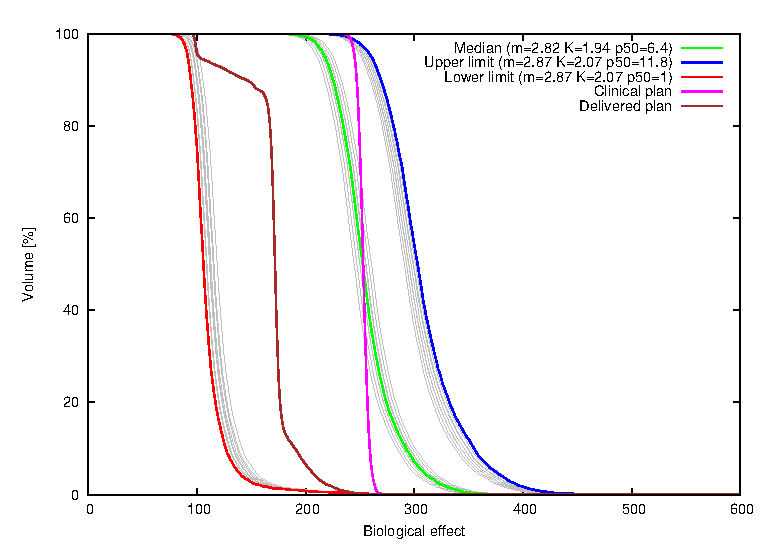
\includegraphics[scale = 1.2]{/Users/alex/Master/contents/images/eDVHRobust.eps}
\vspace{1cm}
\caption{Impact of model parameters uncertainties on the eDVH for patient 1 based on the approved biological dose painted plan with mean values for $K$, $m$ and $p_{50}$.}
\label{fig:eDVHRobust}
\end{figure}
\section{Discussion}
When evaluated with uncertainties, the deployed model shows large differences in HRF distributions, which then lead to different hypoxia tumour maps. In comparison to the tumour map from the plan with mean parameter values, these maps represent scenarios, where the ignorance toward model uncertainties create an over or under estimation of oxygen partial pressures. If the tumour map derived from mean model parameters over estimates the HRF, then dose escalations are set too high in the optimization leading to bad treatment plans. On the other hand, if the mean plan underestimated oxygen partial pressures, dose escalations will not reach the level that is needed to achieve the anticipated biological effect. However, it should be pointed out, that in both cases (over and underestimation of HRF) do not lead to a worse treatment plan than the clinical plan. This is due the fact, that the HRF values can never be lower than 1. Therefore, dose painting can only increase tumour control probability as it only increases (and never decreases) the dose value in a voxel based on the hypoxia map.\\The largest impact on the HRF distributions is due to the large error on the $p_{50}$ parameter from the pO2 model derived by \textit{Chang et al.} as it has a big impact on the range of pO2 value extrapolated from the PET FMISO image. As the $m$ and $K$ parameters only show a small error, which 8 times smaller than the one on $p_{50}$. Therefore it would be desirable to obtain a better measurement on this parameter. 
\section{Conclusion}
The model used in this thesis for the calculation of dose escalations based on FMISO PET images lacks clear robustness as the error on the $p_{50}$ parameter of the pO2 model from \textit{Chang et al.}\cite{pmid19994538} is extremely large. This leads to a wide range of possible HRF distributions that determine the dose escalations in hypoxic volumes. Other sophisticated pO2 models or a better measurement of the $p_{50}$ value would increase the robustness of biological dose painting. However biological dose painting does not create plans that are worse than the clinical plan, as the HRF is limited to values larger than 1.

\chapter{Outlook: Improving Biological Dose Painting}\label{chapter:6}
% chapter 6: improving current dose painting

\section{Understanding PET images}
This chapter deals with the limitations of PET imaging to generate hypoxia tumour maps and will discuss possible improvements that can increase feasibility of biological dose painting.
\subsection{Accuracy of PET images}\label{chap:petaccuracy}
The resolution of PET images in clinical use is about X mm. As the characteristic scale for the transport distance of oxygen through tumour volumes is about X mm, this means that PET is not able to map the microenvironmental oxygen distributions of oxygen. Therefore, PET images only show a mean value of the underlying biology. \textit{Christian et al} \cite{pmid19097661, pmid19293465} showed in a study, how the limitations of PET imaging change biological adaptive IMRT assessed in animal models for FDG by comparing a PET image with an autoradiograph image (resolution of 100$\mu$m). After registration both images were segmented on a threshold-based method, that allowed the creation of equal analysis volumes for both images. The comparison between both images showed that PET images have a low matching value (39\%) when compared to autoradiograph images. The lower the threshold was set to create smaller analysis volumes, the matching value increased. Therefore, higher PET resolution can improve the matching to an autoradiograph image.\\In general PET images show larger discrepancies to the underlying microscopic reality which can be represented with an autoradiograph image. The differences between both images are caused by the lower resolution of PET images. This can also be very important when analyzing small tumour regions that exhibit low oxygen partial pressures. For tumours considered in this work this could also apply for the volumes that show an oxygen partial pressure of 2.5 mmHg. Therefore it can be concluded that higher resolution PET images are necessary to increase the feasibility of biological dose painting.
\subsection{Temporal variance}
As seen in chapter \ref{chapt:chronicacute}, hypoxia can be categorized into chronic and acute hypoxia. Chronic hypoxia is a steady state, that does barely change on a larger time scale, while acute hypoxia exhibits larger fluctuations on the same time scale \cite{pmid9783887, pmid18086391,pmid19203843 - pmid17674980, pmid18313529}. The largest problem with acute hypoxia for biological dose painting is that the hypoxic state of tumour volumes is derived from the PET intensity which is directly correlated to the retention of the hypoxia tracer. As biological dose painting should only target chronic hypoxia, the existence of acute hypoxia leads to an underestimation of the current oxygen partial pressure. This has a direct impact on the HRF distribution and dose escalations, as HRF will be higher in these regions. Of course, this fact only leads to an increased dose in this volume, which does not decrease tumour control but could lead to a scenario, where dose painting could not become feasible as OAR constraints limit the dose delivery. The Wang model \cite{pmid19928070} could enable biological dose painting to give an estimate on the fraction of acute hypoxia. For this approach two PET images are need in a specific time interval to evaluate the changes of oxygenation through FMISO.
\subsection{Reoxygenation \& single image planning}
When tumour cells are damage by ionizing radiation reoxygenation sets in as part of the repair process. This means, that multiple regions in the tumour could have a higher oxygen partial pressure, than assessed with the initial PET image which was used to create the treatment plan. Therefore, the dose requirements to achieve local tumour control with biological dose painting could be decreased by assessing reoxygenation by multiple PET images after a number of fractions. Ideally a new PET image should be the basis for every fraction, to assess tumour hypoxia in every step of the radiation treatment. This approach is not feasible in terms of dose (as PET imaging also introduces a dose to the patient) and treatment costs. As significant reoxygenation seems to be measurable after a certain amount of dose (cf. \ref{tab:po2parameter}), it could be feasible to reassess the initial tumour map after each 10-15 fractions. This could improve the feasibility of dose painting, as hypoxia states are reevaluated and dose escalations are adapted to updated tumour environment. 
\section{Interpretation of hypoxia}
As seen in chapter \ref{chap:hypoxiacorrelation}, correlations between Eppendorf measurements and PET images have been investigated. Nevertheless, most studies have not been able to secure a clear relation between PET SUV and hypoxia for FMISO or other hypoxia tracers. It would be desirable to create a study to systematically investigate the real correlation of PET images and underlying oxygen partial pressures. This can help to understand with the interpretation of PET images and their implementation into the biological dose painting framework discussed in this work.\\As discussed in chapter \ref{chap:petaccuracy} PET images are not able to map the microenvironment with due regard to hypoxia. In a study conducted by \textit{Petit et al.}\cite{pmid19293465} such microenvironmental influences on an intra-voxel basis were evaluated on a similar dose painting model as implemented in this work. The microenvironmental distribution of oxygen can lead to higher radioresistance as compared to homogeneous cellular pO2 distributions. This can lead to a median gain in cell kill when adapted to the biological dose painting approach of this work. One major drawback of a intra-voxel microenvironment distribution derived from PET is related to the changes introduces by reoxygenation of tumour volumes during radiotherapy. A closer investigation on the influence of intra-voxel distributions in terms of reoxygenation could help understand the complex approach of dynamic dose painting based on multiple PET images.
%\section{Role of prescriptions}
%Dose escalations in the deployed model in biological dose painting are calculated based on an initial prescription, which is derived from the clinical plan. The dose prescriptions to tumour volumes are a combination of empirical values from in vivo and in vitro investigations and the experience of the radiation therapist. The feasibility of dose painting depends on the dose prescriptions set in the tumour volume. It is questionable if such prescriptions are beneficial for dose painting. Therefore this work proposes a new way dose painting called \textit{prescription free biological dose painting} (PFBDP). Rather than basing the dose delivery on initial prescriptions in tumour volumes (e.g. 70 Gy), this approach will only incorporate dose limits for all critical structures.

\chapter{Summary \& Conclusions}\label{chapter:X}

\newpage
\setcounter{page}{1}
\pagenumbering{roman}

\appendix
\chapter{Dose compensation for hypoxia}%
As hypoxia will decrease radio sensitivity the dose has to be increased to achieve the same biological effect. The reference effect is derived from the prescribed dose $D_p$ with $\varepsilon_p = \alpha_X D_p + \beta_X D_p^2$. The compensating dose $D$ to overcome the effects of hypoxia is
\begin{equation}
\underbrace{\alpha_X D_p + \beta_X D_p}_{=\varepsilon_p} \mathop{=}\limits^! \frac{\alpha_X}{\mathrm{HRF}} D + \frac{\beta_X}{\mathrm{HRF}^2} D^2\\
\end{equation}
Bringing this into a solvable quadratic form yields
\begin{eqnarray}
\frac{\alpha_X}{\mathrm{HRF}} D + \frac{\beta_X}{\mathrm{HRF}^2} D^2 - \varepsilon_p  &=& 0\\
D^2 + \mathrm{HRF}\cdot\frac{\alpha_X}{\beta_X}\cdot D - \frac{\mathrm{HRF}^2}{\beta_X}\varepsilon_p &=& 0.
\end{eqnarray}
The two solutions to this equation are
\begin{equation}
D_{1,2} = \mathrm{HRF}\left[-\frac{\alpha_X}{2\beta_X} \pm \sqrt{\left(\frac{\alpha_X}{2\beta_X}\right)^2 + \frac{\varepsilon_p}{\beta_X}}\right]
\end{equation}
The negative solution is dropped as it generated a negative dose result and is therefore unphysical. Dose is linearly scaled up with the HRF to compensate for hypoxia and achieve the prescribed effect $\varepsilon_p$. \label{appendix:a}
\chapter{Patient statistics}%
All patients presented in this thesis have been provided with a clinical plan approved by a physician or radiation oncologist. All plans follow the HN06 trail dose constraints. Due to the incomparability of patients treatment volumes, every patient is presented with his own table.

% pat 1 pat 2 
\begin{sidewaystable}[p]
\hspace{1cm}
\subfigure[Patient 1]{
 \centering
 \footnotesize
 \begin{tabular}{ccccc}
 \toprule
 \multicolumn{1}{c}{Patient 1} & \multicolumn{2}{c}{Clinical plan [Gy]}  & \multicolumn{2}{c}{Biological dose painting [Gy]}\\
 \cmidrule(r){1-1} \cmidrule(r){2-3}\cmidrule(r){4-5}
 Volume name & $D_\mathrm{mean}$ & $D_\mathrm{max}$ & $D_\mathrm{mean}$ & $D_\mathrm{max}$\\
 \midrule\\
 BRAIN & 14.13 & 75.18 & 12.62 & 76.65 \\
 BRSTEM & 19.96 & 52.06 & 17.93 & 48.63 \\
 CHIASM & 16.27 & 23.04 & 10.49 & 12.46 \\
 CORD & 15.25 & 42.93 & 15.32 & 44.56 \\
 ESOPHAGUS & 22.53 & 53.51 & 20.93 & 50.06 \\
 LARYNX & 40.20 & 66.07 & 29.07 & 64.00 \\
 LEYE & 6.39 & 17.01 & 4.72 & 18.92 \\
 LIPS & 17.94 & 50.01 & 26.72 & 41.30 \\
 LLENS & 5.29 & 6.52 & 3.60 & 4.80 \\
 LNECK & 40.62 & 77.64 & 50.90 & 115.46 \\
 LOPTIC & 14.55 & 34.01 & 9.26 & 19.42 \\
 LPAROTID & 38.62 & 74.63 & 65.8 & 85.5 \\
 LPLEXUS & 32.02 & 67.39 & 30.95 & 67.32 \\
 MANDIBLE & 42.03 & 75.01 & 39.40 & 74.74 \\
 POSTCRICOID & 44.26 & 62.37 & 35.80 & 59.17 \\
 REYE & 5.59 & 11.73 & 4.68 & 14.38 \\
 RLENS & 4.39 & 5.78 & 4.10 & 6.95 \\
 RNECK & 39.67 & 77.33 & 50.32 & 89.11 \\
 ROPTIC & 10.60 & 17.71 & 8.55 & 11.74 \\
 RPAROTID & 34.53 & 75.19 & 34.26 & 77.37 \\
 RPLEXUS & 30.42 & 65.96 & 27.40 & 66.83 \\\\
 \bottomrule\\
 CTV56 & 60.28 & 78.49 & 76.2 & 119.8 \\
 CTV70 & 68.47 & 78.49 & 81.1 & 119.8 \\
 GTV & 68.94 & 78.49 & 93.4 & 119.8 \\
 GTV50 & - & - & 95.5 & 119.8 \\
 GTV25 & - & - & 92 & 119.8 \\
 PTV56 & 34.87 & 78.49 & 71.7 & 119.8 \\
 PTV70 & 61.54 & 78.49 & 76.3 & 119.8 \\\\
 \bottomrule\\
 \end{tabular}
}
\hspace{0.5cm}
\subfigure[Patient 2]{
 \centering
 \footnotesize
 \begin{tabular}{ccccc}
 \toprule
 \multicolumn{1}{c}{Patient 1} & \multicolumn{2}{c}{Clinical plan [Gy]} & \multicolumn{2}{c}{Biological dose painting [Gy]}\\
 \cmidrule(r){1-1} \cmidrule(r){2-3}\cmidrule(r){4-5}
 Volume name & $D_\mathrm{mean}$ & $D_\mathrm{max}$ & $D_\mathrm{mean}$ & $D_\mathrm{max}$\\
 \midrule\\
BRSTEM & 16.47 & 43.68 & 12.09 & 42.03 \\
CHIASM & 4.15 & 5.11 & 2.22 & 3.18 \\
CORD & 17.76 & 45.03 & 14.19 & 40.79 \\
ESOPHAGUS & 22.18 & 57.80 & 12.50 & 38.50 \\
LARYNX & 43.30 & 65.54 & 21.61 & 58.98 \\
LEYE & 2.42 & 5.51 & 1.60 & 3.00 \\
LIPS & 16.05 & 39.85 & 11.21 & 26.67 \\
LLENS & 2.68 & 3.58 & 1.41 & 1.59 \\
LOPTIC & 4.23 & 5.36 & 2.14 & 3.18 \\
LPLEXUS & 29.85 & 72.07 & 25.65 & 64.10 \\
MANDIBLE & 44.23 & 74.50 & 29.65 & 67.63 \\
POSTCRICOID & 44.65 & 62.94 & 25.99 & 58.98 \\
RACOUSTIC & 28.84 & 55.83 & 11.73 & 29.14 \\
REYE & 2.12 & 4.59 & 1.59 & 2.47 \\
ROPTIC & 3.77 & 4.79 & 1.92 & 2.65 \\
RPAROTID & 51.55 & 75.32 & 39.23 & 74.52 \\\\\\\\\\\\\\
 \bottomrule\\
CTV56 & 68.59 & 76.32 & 71.20 & 88.30 \\
CTV70 & 71.27 & 76.32 & 74.60 & 88.30 \\
GTV & 72.19 & 76.32 & 81.90 & 88.30 \\
GTV50 & - & - & 84.30 & 88.30 \\
GTV25 & - & - & - & - \\
PTV56 & 62.97 & 76.32 & 67.30 & 88.30 \\
PTV70 & 68.56 & 76.32 & 71.20 & 88.30 \\\\
 \bottomrule\\
 \end{tabular}
}
\end{sidewaystable}

% pat 3 pat 4 

\begin{sidewaystable}[p]
\hspace{1cm}
\subfigure[Patient 3]{
 \centering
 \footnotesize
 \begin{tabular}{ccccc}
 \toprule
 \multicolumn{1}{c}{Patient 1} & \multicolumn{2}{c}{Clinical plan [Gy]}  & \multicolumn{2}{c}{Biological dose painting [Gy]}\\
 \cmidrule(r){1-1} \cmidrule(r){2-3}\cmidrule(r){4-5}
 Volume name & $D_\mathrm{mean}$ & $D_\mathrm{max}$ & $D_\mathrm{mean}$ & $D_\mathrm{max}$\\
 \midrule\\
BRAIN & 10.64 & 54.39 & 7.50 & 54.18 \\
BRSTEM & 13.61 & 42.36 & 11.72 & 41.60 \\
CHIASM & 2.75 & 3.18 & 2.11 & 3.14 \\
CORD & 15.71 & 38.51 & 12.36 & 37.01 \\
ESOPHAGUS & 34.70 & 72.31 & 31.07 & 71.35 \\
LEYE & 1.34 & 4.05 & 1.08 & 2.66 \\
LIPS & 13.72 & 30.34 & 14.84 & 27.82 \\
LLACRIMAL & 1.56 & 3.04 & 0.88 & 1.45 \\
LLENS & 1.27 & 2.21 & 1.31 & 1.94 \\
LOPTIC & 2.93 & 3.38 & 1.72 & 2.66 \\
LPAROTID & 40.94 & 76.24 & 33.48 & 74.74 \\
LPLEXUS & 26.93 & 66.56 & 25.91 & 63.85 \\
MANDIBLE & 34.43 & 73.87 & 47.60 & 75.90 \\
REYE & 2.13 & 6.99 & 1.32 & 4.60 \\
RLACRIMAL & 2.02 & 3.10 & 1.14 & 1.94 \\
RLENS & 2.22 & 3.10 & 1.31 & 1.94 \\
ROPTIC & 3.13 & 3.64 & 2.28 & 2.90 \\
RPAROTID & 43.82 & 75.24 & 40.46 & 75.46 \\
RPLEXUS & 29.89 & 72.13 & 31.46 & 72.32 \\\\
\bottomrule\\
CTV56 & 60.55 & 76.94 & 77.90 & 120.90 \\
CTV70 & 69.96 & 76.52 & 81.60 & 120.90 \\
GTV & 71.12 & 76.47 & 88.90 & 120.90 \\
GTV50 & - & - & 94.40 & 120.90 \\
GTV25 & - & - & 104.60 & 120.90 \\
PTV56 & 35.33 & 76.94 & 72.60 & 120.90 \\
PTV70 & 36.08 & 76.94 & 76.90 & 120.90 \\\\
 \bottomrule\\
 \end{tabular}
}
\hspace{0.5cm}
\subfigure[Patient 4]{
 \centering
 \footnotesize
 \begin{tabular}{ccccc}
 \toprule
 \multicolumn{1}{c}{Patient 1} & \multicolumn{2}{c}{Clinical plan [Gy]} & \multicolumn{2}{c}{Biological dose painting [Gy]}\\
 \cmidrule(r){1-1} \cmidrule(r){2-3}\cmidrule(r){4-5}
 Volume name & $D_\mathrm{mean}$ & $D_\mathrm{max}$ & $D_\mathrm{mean}$ & $D_\mathrm{max}$\\
 \midrule\\
BRAIN & 12.15 & 55.43 & 8.28 & 53.08 \\
BRSTEM & 14.96 & 39.21 & 10.63 & 33.06 \\
CORD & 15.91 & 38.47 & 13.85 & 39.36 \\
ESOPHAGUS & 26.20 & 54.91 & 23.30 & 50.61 \\
HYPOPHARYNX & 47.61 & 72.13 & 48.02 & 68.60 \\
LARYNX & 47.57 & 74.76 & 44.25 & 68.37 \\
LPAROTID & 23.06 & 63.33 & 22.50 & 58.48 \\
MANDIBLE & 28.71 & 71.91 & 26.95 & 70.85 \\
RPAROTID & 26.03 & 72.12 & 31.21 & 68.37 \\\\\\\\\\\\\\\\\\\\\\\\
\bottomrule\\  
CTV56 & 66.48 & 76.85 & 71.60 & 112.50 \\
CTV70 & 68.50 & 76.85 & 74.40 & 112.50 \\
GTV & 71.39 & 76.78 & 80.00 & 112.50 \\
GTV50 & - & - & 86.00 & 112.50 \\
GTV25 & - & - & 96.80 & 112.50 \\
PTV56 & 59.00 & 76.85 & 67.70 & 112.50 \\
PTV70 & 65.40 & 76.85 & 71.20 & 112.50 \\\\
 \bottomrule\\
 \end{tabular}
}
\end{sidewaystable}

% pat 5 pat 6 

\begin{sidewaystable}[p]
\hspace{1cm}
\subfigure[Patient 5]{
 \centering
 \footnotesize
 \begin{tabular}{ccccc}
 \toprule
 \multicolumn{1}{c}{Patient 1} & \multicolumn{2}{c}{Clinical plan [Gy]}  & \multicolumn{2}{c}{Biological dose painting [Gy]}\\
 \cmidrule(r){1-1} \cmidrule(r){2-3}\cmidrule(r){4-5}
 Volume name & $D_\mathrm{mean}$ & $D_\mathrm{max}$ & $D_\mathrm{mean}$ & $D_\mathrm{max}$\\
 \midrule\\
BRAIN & 10.44 & 53.75 & 5.42 & 44.52 \\
BRSTEM & 16.65 & 49.23 & 11.74 & 44.75 \\
CHIASM & 3.09 & 3.58 & 2.11 & 3.03 \\
CORD & 17.83 & 43.31 & 14.97 & 44.05 \\
ESOPHAGUS & 25.75 & 58.55 & 18.65 & 55.24 \\
LARYNX & 50.06 & 71.77 & 38.94 & 68.76 \\
LEYE & 2.32 & 6.27 & 1.48 & 3.73 \\
LIPS & 16.75 & 57.99 & 27.65 & 50.81 \\
LLACRIMAL & 2.37 & 2.91 & 1.24 & 1.87 \\
LLENS & 2.56 & 3.33 & 1.45 & 1.87 \\
LNECK & 57.64 & 75.84 & 52.04 & 75.52 \\
LOPTIC & 3.54 & 4.19 & 2.20 & 3.50 \\
LPAROTID & 33.20 & 75.74 & 32.75 & 67.36 \\
LPHARYNGEAL & 62.12 & 72.91 & 52.79 & 72.02 \\
MANDIBLE & 37.41 & 74.39 & 38.08 & 75.05 \\
REYE & 2.96 & 6.96 & 1.82 & 4.20 \\
RLACRIMAL & 2.81 & 3.67 & 1.62 & 2.33 \\
RLENS & 2.99 & 3.66 & 1.80 & 2.56 \\
RNECK & 54.13 & 76.20 & 44.39 & 82.51 \\
ROPTIC & 3.74 & 4.45 & 2.41 & 3.26 \\
RPAROTID & 29.44 & 73.20 & 34.81 & 67.36 \\
RPHARYNGEAL & 61.55 & 73.29 & 50.33 & 75.75 \\\\
\bottomrule\\
CTV56 & 42.57 & 77.35 & 73.00 & 116.60 \\
CTV70 & 46.45 & 77.35 & 76.60 & 116.60 \\
GTV & 69.81 & 77.00 & 85.50 & 116.60 \\
GTV50 & - & - & 91.20 & 116.60 \\
GTV25 & - & - & 100.70 & 116.60 \\
PTV56 & 35.30 & 77.35 & 71.70 & 116.60 \\
PTV70 & 35.97 & 77.35 & 68.10 & 116.60 \\\\
 \bottomrule\\
 \end{tabular}
}
\hspace{0.5cm}
\subfigure[Patient 4]{
 \centering
 \footnotesize
 \begin{tabular}{ccccc}
 \toprule
 \multicolumn{1}{c}{Patient 1} & \multicolumn{2}{c}{Clinical plan [Gy]} & \multicolumn{2}{c}{Biological dose painting [Gy]}\\
 \cmidrule(r){1-1} \cmidrule(r){2-3}\cmidrule(r){4-5}
 Volume name & $D_\mathrm{mean}$ & $D_\mathrm{max}$ & $D_\mathrm{mean}$ & $D_\mathrm{max}$\\
 \midrule\\
BRAIN & 15.93 & 77.36 & 10.02 & 75.23 \\
BRSTEM & 29.12 & 55.76 & 20.84 & 50.08 \\
CHIASM & 30.59 & 51.82 & 14.70 & 32.61 \\
CORD & 17.23 & 41.62 & 15.03 & 41.92 \\
ESOPHAGUS & 35.76 & 74.35 & 27.06 & 69.64 \\
LACOUSTIC & 34.22 & 50.04 & 29.80 & 42.86 \\
LARYNX & 46.62 & 74.23 & 34.44 & 72.20 \\
LEYE & 2.87 & 7.52 & 1.42 & 4.43 \\
LIPS & 14.50 & 42.47 & 11.93 & 37.50 \\
LLACRIMAL & 3.06 & 4.75 & 1.15 & 2.10 \\
LLENS & 3.29 & 3.91 & 1.23 & 1.63 \\
LOPTIC & 17.92 & 43.16 & 7.67 & 20.50 \\
LPAROTID & 37.38 & 76.52 & 27.38 & 68.71 \\
MANDIBLE & 44.60 & 73.74 & 33.41 & 69.87 \\
POSTCRICOID & 51.11 & 75.17 & 37.26 & 72.67 \\
RACOUSTIC & 39.95 & 49.49 & 28.67 & 46.58 \\
REYE & 4.55 & 15.51 & 2.10 & 7.45 \\
RLACRIMAL & 4.50 & 8.95 & 1.48 & 2.80 \\
RLENS & 3.94 & 5.01 & 1.54 & 2.10 \\
ROPTIC & 19.60 & 45.38 & 9.85 & 24.46 \\
RPAROTID & 46.79 & 74.75 & 32.18 & 72.67 \\\\\\
\bottomrule\\       
CTV56 & 41.55 & 78.02 & 75.60 & 116.50 \\
CTV70 & 60.76 & 78.02 & 80.90 & 116.50 \\
GTV & 63.50 & 77.03 & 86.90 & 116.50 \\
GTV25 & - & - & 93.40 & 116.50 \\
GTV50 & - & - & 102.80 & 116.50 \\
PTV56 & 34.84 & 78.02 & 68.90 & 116.50 \\
PTV70 & 35.71 & 78.02 & 74.80 & 116.50 \\\\
 \bottomrule\\
 \end{tabular}
}
\end{sidewaystable}\label{appendix:b}

%\newpage
%\glsaddall
%\renewcommand{\glsgroupskip}{}
%\printglossary[type=\acronymtype,style=long,title=Table of Acronyms]

%\newpage
%\printglossary[style=altlist,title=Glossary]

\cleardoublepage
\phantomsection
\addcontentsline{toc}{chapter}{Bibliography}
\nocite{*}
\bibliographystyle{\mybibstyle}
\footnotesize{
 \bibliography{contents/other/references_url.bib}
}

\listoffigures
\listoftables

\end{document} 
